\chapter{物理节点单故障可生存性虚拟网络嵌入算法}
\section{问题描述}
在这一部分中,我们首先介绍了虚拟网络嵌入的基本概念,然后提出了我们的可生存性虚拟网络嵌入问题。
\subsection{虚拟网络嵌入}
我们将\textbf{虚拟网络}VN表示为无向图$G (V,E)$,其中$V$ 和$E$ 分别是虚拟节点和虚拟链路的集合。每个虚拟链路$e_{ij}$具有带宽需求$d_{ij}$。 每个虚拟节点$v_i$ 具有计算容量需求$d_i$。 对于虚拟节点$v_i$,需要在虚拟节点上执行的虚拟功能表示为$f(i)$。如图\ref{fig:VirtualNetworkRequest} 所示虚拟网络$G (V,E)$ 具有虚拟节点集$V=\{v_1,v_2,v_3,v_4\}$ 和虚拟边集$E= \{e_{12},e_{13},e_{14},e_{23}\}$。需要在这些虚拟节点上执行的虚拟函数是$f(1)=f_1$, $f(2)=f_2$, $f(3)=f_3$, $f(4)=f_4$。

\begin{figure}[htbp]
\centering
% Requires \usepackage{graphicx}
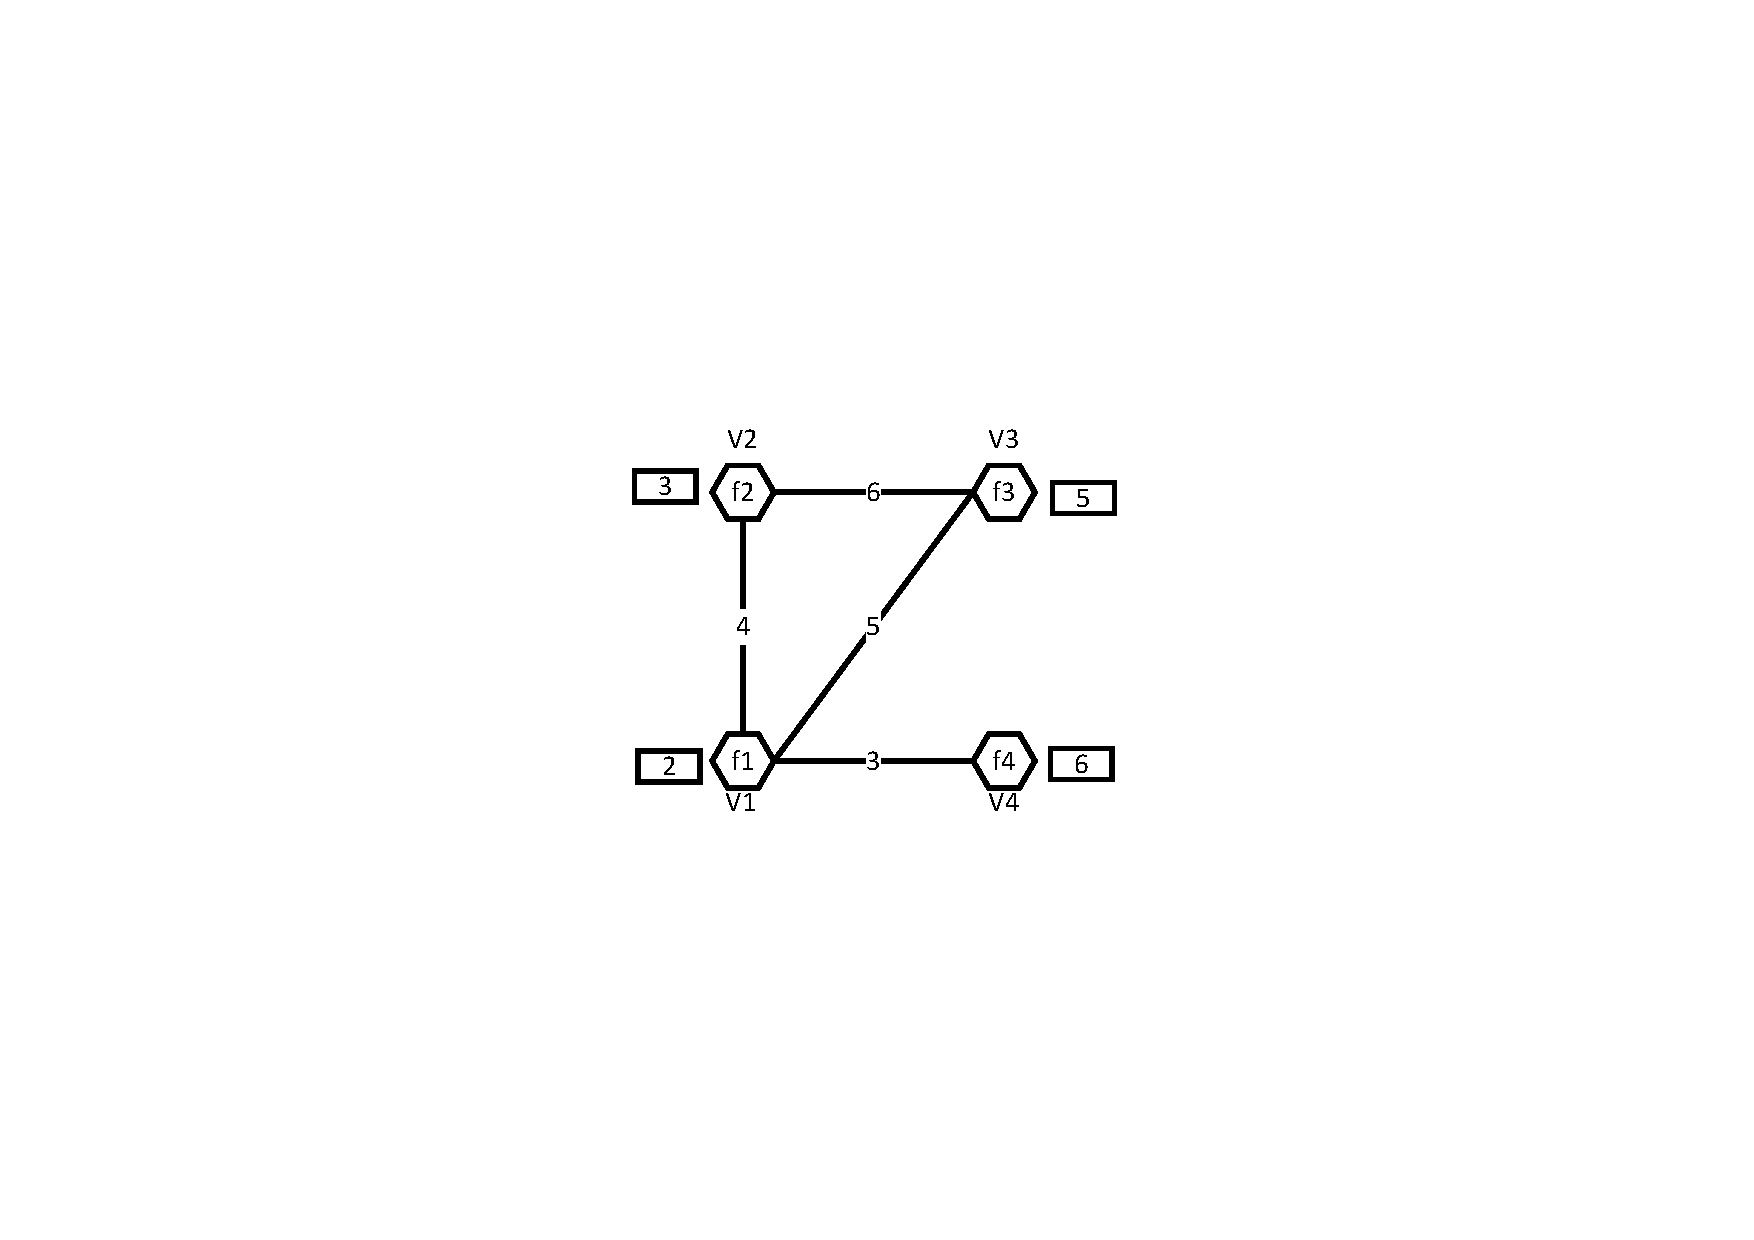
\includegraphics[width=3.0in]{figures/VirtualNetworkRequest}\\
\caption{虚拟网络请求$G(V,E)$
}\label{fig:VirtualNetworkRequest}
\end{figure}

我们将底层\textbf{物理网络}建模为一个无向图$G (S,L)$,其中$S$ 和$L$ 分别是物理节点和物理链路的集合。对于物理节点$s_i$,我们使用$F(i)$ 和$c_i$分别表示可以在该节点上执行的一组可行的虚拟功能和可用的计算能力。每个物理链路$l_{ij}$ 都有可用带宽$b_{ij}$。如图\ref{fig:PhysicalNetwork}所示的物理网络$G (S,L)$,物理节点集合$S=\{s_1,s_2,s_3,s_4,s_5,s_6,s_7,s_8\}$,链路集合$L=\{l_{12},l_{13},l_{14},l_{15},l_{23},l_{25},l_{35},l_{36},l_{37},l_{47},l_{58}\}$,
每一个物理节点的可行的虚拟功能$F(1)=\{f_1\}$, $F(2)=\{f_2,f_3\}$, $F(3)=\{f_3\}$, $F(4)=\{f_4\}$, $F(5)=\{f_1,f_2\}$, $F(6)=\{f_1,f_4\}$, $F(7)=\{f_2,f_3\}$,$F(8)=\{f_2\}$。

\begin{figure}[htbp]
\centering
% Requires \usepackage{graphicx}
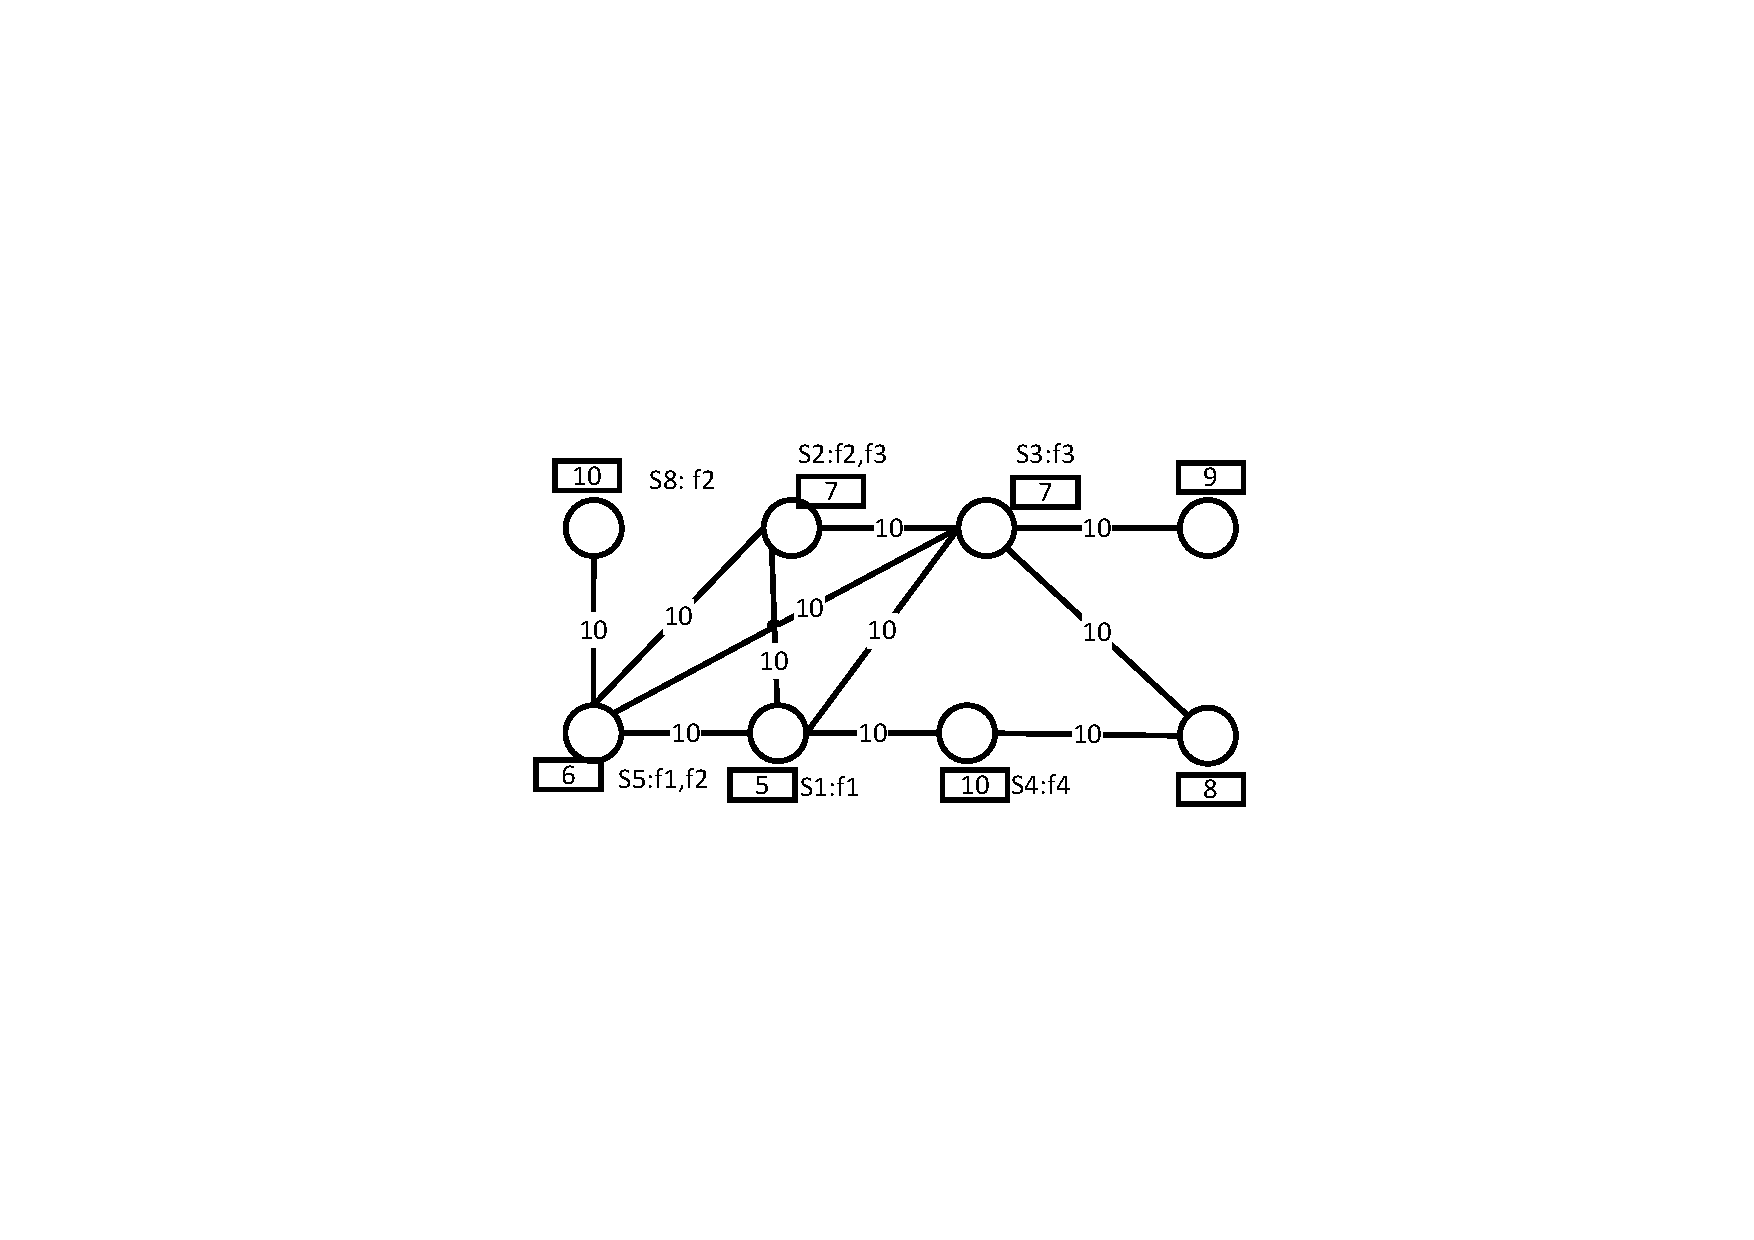
\includegraphics[width=3.8in]{figures/PhysicalNetwork}\\
\caption{底层物理网络$G(S,L)$}\label{fig:PhysicalNetwork}
\end{figure}

在给定VN请求$G (V,E)$的情况下,虚拟网络嵌入问题的目的是将该请求映射到物理网络$G (S,L)$ 上,同时提供所需的足够资源。一个可行的嵌入应该满足节点容量约束、链路带宽约束和功能类型约束这三个约束条件。
对于一个虚拟节点$v_i$,物理节点$s_j$只在节点容量约束和功能类型两种情况满足约束条件(即${f_i} \in {F_j}$)下被映射这个虚拟节点。即节点的容量请求应满足$d_i\leq c_j$的物理节点,虚拟节点上需要执行的虚拟功能属于物理节点$s_j$ 上可以执行的虚拟功能集${f_i} \in {F_j}$。 如果物理节点$s_j$ 满足这两个约束,则节点映射是可行的,并且我们表示这样的映射为$\phi ({v_i}) = {s_j}$。

对于在两个已经映射到两个物理节点$s_{i'}$和$s_{j'}$(即$\phi({v_i}) = {s_{i'}}$ 和$\phi({v_j}) = {s_{j'}}$) 的虚拟节点之间的虚拟链路$e_{ij}$,在链路带宽约束下$d_{ij}\leq b_{i'j'}$(其中$b_{i'j'}$是连接物理节点$s_{i'}$ 和$s_{j'}$的可用带宽),这条虚拟链路$e_{ij}$ 可以映射到物理路径$p_{\phi({v_i}) \phi({v_j})}$,则表示可行的链路映射为$\rho(e_{ij}) = p_{\phi({v_i}) \phi({v_j})}$。

显然,为了找到一个可行的虚拟网络嵌入,我们需要找到两个映射函数$\phi$ 和$\rho$来将所有虚拟节点映射到物理节点,以及将所有虚拟链路映射到物理路径。

如图\ref{fig:VirtualNetworkEmbedding}所示一个可行的虚拟网络嵌入,将图\ref{fig:VirtualNetworkRequest}中的虚拟网络嵌入到图\ref{fig:PhysicalNetwork} 中的物理网络中,其中虚拟节点$v_1$嵌入到物理节点$s_1$,虚拟节点$v_2$嵌入到物理节点$s_2$,虚拟节点$v_3$ 嵌入到物理节点$s_3$,虚拟节点$v_4$嵌入到物理节点$s_4$。 在图\ref{fig:PhysicalNetwork} 中,我们还展示了在这样映射之后物理网络中已经占用的和可用的资源。例如,对于物理节点$s_1$,其占用的计算容量为2,可用容量为5。

给定VN请求$G(V,E)$和物理网络$G(S,L)$,对于可行映射,我们将映射的物理图表示为$G\left( {\hat S,P} \right)$,其中$\hat S$是容纳虚拟节点的物理节点集,其中$\hat S = \{ {s_{i'}}:\phi({v_i}) = {s_{i'}},for\ \ {\rm{ }}all\ {v_i} \in V,{s_{i'}} \in S\}$ 和$P$ 是路径集,其中每个路径都持有一个虚拟链路$P = \{ p_{\phi({v_i}) \phi({v_j})}:\rho(e_{ij}) = p_{\phi({v_i}) \phi({v_j})}{\rm{ }}, for\ all,{e_{ij}} \in E\}$。由于每个虚拟链路对应一个物理网络路径,该路径由多个物理链路组成,因此我们还将$G\left( {\hat S,\hat L} \right)$表示为占领的物理网络$\hat L = \{ {l_{pg}}:{l_{pg}} \in {p_{s_{i'}s_{j'}}}, \rho(e_{ij}) = p_{\phi({v_i}) \phi({v_j})},for\ all\ {e_{ij}} \in E,{l_{pg}} \in L\}$。

已经有了许多关于虚拟网络嵌入问题\cite{fischer2013virtual}的研究;,因为本文的重点不是虚拟网络嵌入算法,我们采用了\cite{lischka2009virtual} 中的算法作为基本的虚拟网络嵌入算法。


\begin{figure}[htbp]
\centering
% Requires \usepackage{graphicx}
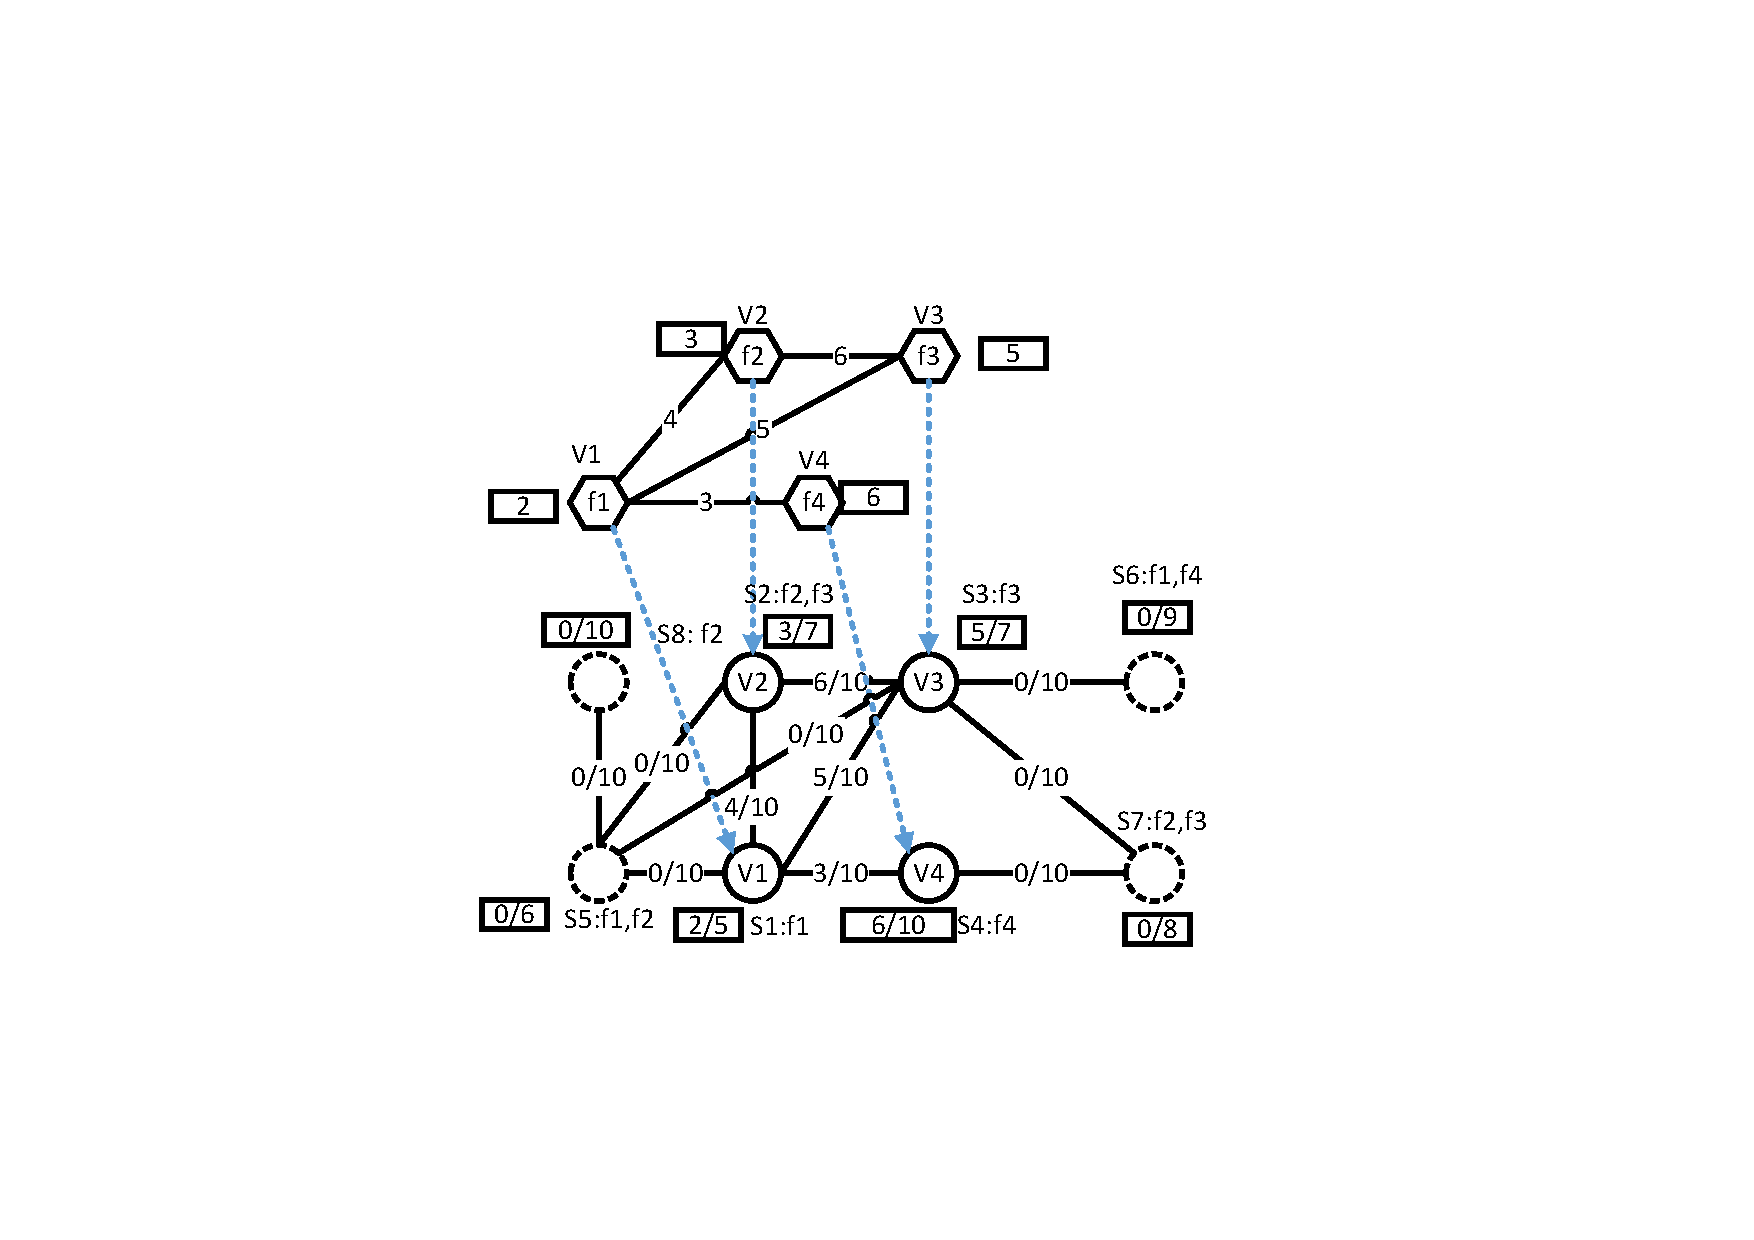
\includegraphics[width=4in]{figures/VirtualNetworkEmbedding}\\
\caption{节点映射和链路映射的实例}\label{fig:VirtualNetworkEmbedding}
\end{figure}
\subsection{可生存性虚拟网络嵌入}
由于恶意攻击、自然灾害、无意中断电缆、计划维护、设备故障、物理节点承载的虚拟节点可能会遭受不可避免的故障。当单个或多个物理网络组件发生故障时,VN 中可能会发生故障,从而造成财务损失。一般来说,多个物理节点的同时失效是相互独立的,单个节点的失效通常发生在大多数时间\cite{yeow2010designing}。本文研究了单节点失效的可生存性虚拟网络嵌入问题。在本章中,我们将讨论如何将我们的算法扩展到多节点故障的场景中。

对于VN请求$G (V,E)$和物理网络$G (S,L)$,给出了其占用物理网络的可行映射,在任何一个物理节点发生故障时,增加最小备份物理资源以提供可生存性的网络服务。

节点故障不仅影响运行在失效的物理节点上的可视化服务,而且会终止通过该节点的所有通信。物理节点 $ {s_i} \in S $ 的失效导致相邻物理链路的失效${L_i} = \left\{ {{l_{ik}}:k \in N(i)} \right\}$,其中${N(i)}$ 是节点$ {s_i} $的邻居节点。物理链路的失效场景可以通过增加中间节点的方法等价转换为节点故障的场景。

由于我们无法预测哪个节点将失效,即使我们知道多个节点不会同时失效,为了处理单节点故障,一个直接的方式是为VN请求中的每个虚拟节点提供专用备份资源,也称为1+1 保护方案。如图\ref{fig:One2OneProtection}所示利用一个例子来说明这种直截了当的方法。在该示例中,将具有4个虚拟节点的虚拟网络映射到物理网络,其中4 个物理节点参与了这样的嵌入。为了提供1 +1 保护方案,在图中添加了4 个备份节点、8 个备份链路。

1+1保护方案虽然实现简单,但需要大量的备份资源提去算法的目的是以最小的备份资源成本提供可生存性的网络服务。

\begin{figure}[htbp]
\centering
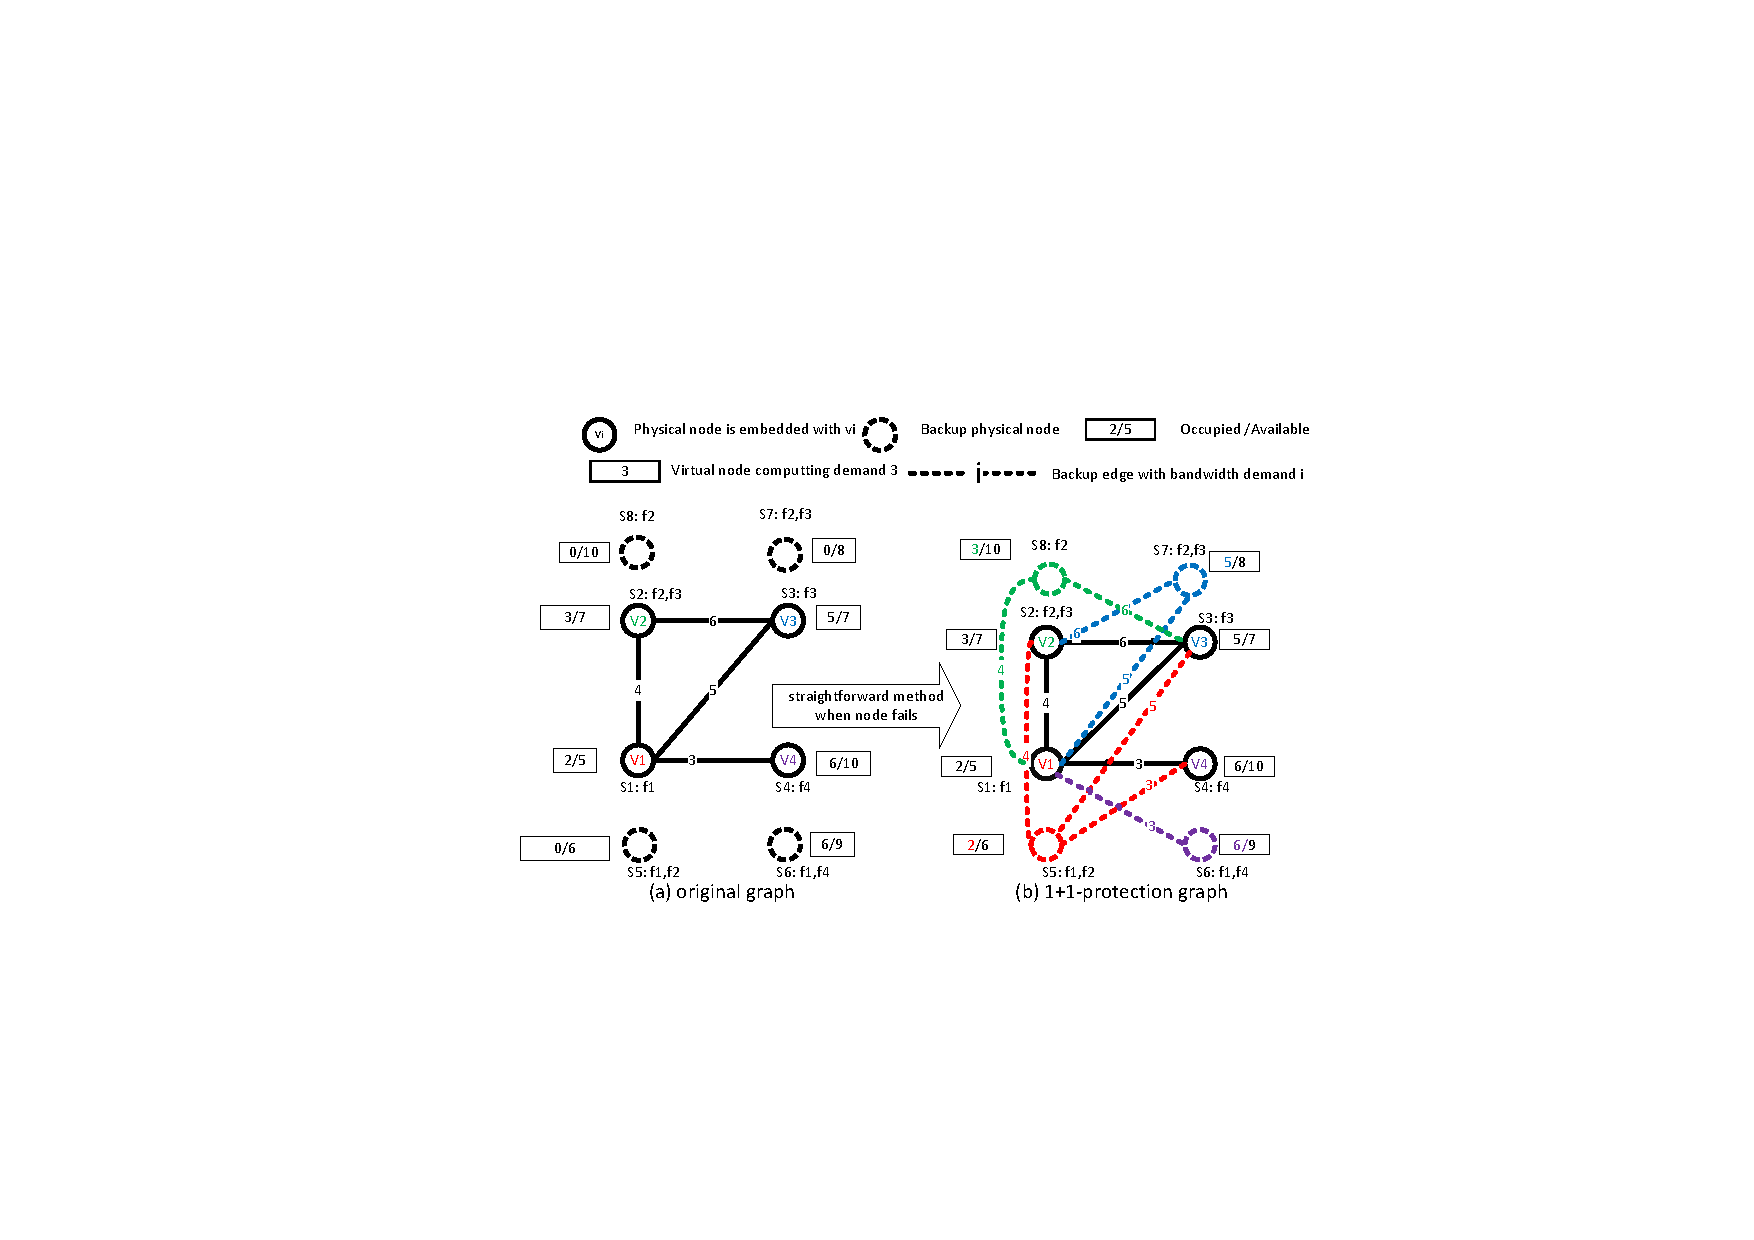
\includegraphics[width=4.5in]{figures/One2OneProtection}\\
\caption{1+1-保护机制}\label{fig:One2OneProtection}
\end{figure}
\section{图分解}
可生存性虚拟网络嵌入需要添加备份资源,以保证当任何一个物理节点失效时,剩余的物理资源加上备份资源仍然可以支持原先的虚拟网络请求。为了便于在节点失效时找到可行的嵌入,本节首先对虚拟网络进行分解,物理网络以星型结构为基础的局部组件。在此基础上,提出了一种新的二分图,并将具有最小备份资源的可生存性虚拟网络嵌入问题转化为一个基于定义良好的二分图的虚拟星图分配问题。
\subsection{基于星型图的分解}
将虚拟网络分解为虚拟局部星型图。每个虚拟局部星型图与一个虚拟节点相关联。给出虚拟节点$v_i$,相应的虚拟局部星型图被定义为属性化单层根树,并如公式\ref{eq:virtualstar} 所示。

\begin{equation}
VirtualStar(v_i)=(v_i, \phi(v_i), d_i, f_i, D_i, N_i)
\label{eq:virtualstar}
\end{equation}


其中,$N_i$是虚拟网络中的相邻节点集,并与节点$v_i$相关联的带宽需求集${D_i} = \left\{ {{d_{ij}}|{v_j} \in {N_i}} \right\} $。 注意,VirtualStar($v_i$) 包括节点映射信息$\phi(v_i)$。 因为我们希望最小化备份资源以提供可生存性的网络服务,在节点失效前重复使用映射可能减少额外资源,使系统保持稳定的一个很好的选择。在虚拟星型图结构中,根节点和它的邻居节点存在链路,但是根节点的邻居节点之间不存在链路。

物理网络被分解为物理局部星型图。同样,每个物理局部星型图与一个物理节点相关联。给定物理节点$s_j$,对应的物理局部星型图被定义为属性化单层根树,并表示如公式\ref{eq:physicalstar}所示。
\begin{equation}
PhysicalStar(s_j)=(s_j, \phi^{-1}( s_j), c_j, F(j), \phi(N(\phi^{-1}( s_j))), a)
\label{eq:physicalstar}
\end{equation}

其中$\phi^{-1}( s_j)$是映射到物理节点$s_j$的虚拟节点集,$N(\phi^{-1}( s_j))$ 是$\phi^{-1}( s_j)$中虚拟节点的相邻节点,$\phi(N(\phi^{-1}( s_j)))$ 是承载这些邻居的物理节点,$c_j$是节点容量,$F(j)$ 是$s_j$支持的虚拟功能,$a$是一个1 位的单比特,它的值为0 或1,以指示这个物理节点是否开启和设置了虚拟机。与虚拟星型图类似,在物理星型图结构中,根节点与相邻节点之间存在边,相邻节点之间不存在边。定义在\ref{eq:virtualstar} 和\ref{eq:physicalstar} 中的虚拟星型图和物理星型图很好地捕获了隐藏在VN 请求中的局部结构,以保持节点与其相邻节点之间的关系。基于虚拟局部星型图和物理虚拟星型图,虚拟网络和物理网络可以分解为多个组件。

\subsection{二分图}
构造了一个二分图$G=\{V_1,V_2,E\}$来表示虚拟网络与物理网络之间的关系。$V_1$ 和$V_2$分别表示虚拟星型图和物理星型图的集合。如果VirtualStar($v_i$) 的虚拟功能 $f_i$能在具有${f_i} \in {F_j}$ 的物理节点$s_j$上执行,则在边集$E$ 中添加边$e(i,j)$,以连接VirtualStar($v_i$) 和PhysicalStar($s_j$)。

我们的目标是最小化备份资源以提供可生存性的服务。为了服务于目标,给定边$e(i,j)$,我们定义了边权$w(i,j)$作为备份资源成本。当节点发生故障时,将虚拟星型图($v_i$) 映射到物理星型图($s_j$)。 根据虚拟节点$v_i$映射到物理节点$s_j$ 节点是否失效,如公式\ref{eq:edge weight}所示在两种不同的情况下定义了边权重$w(i,j)$。
\begin{equation}
w(i,j) = \left\{ {\begin{array}{*{20}{c}}
   { \alpha \sum\limits_{\phi ({v_k}) \notin \phi (N({\phi ^{ - 1}}({s_j})))} {{d_{ik}}} } & {{v_i} \in {\phi ^{ - 1}}({s_j}),v_k \in N(i)}  \\
   {\alpha \sum\limits_{k \in N(i)} {{d_{ik}}}  + \beta {M_m} + \lambda {c_i} + \theta } & {{v_i} \notin {\phi ^{ - 1}}({s_j}),v_k \in N(i)}  \\
\end{array}} \right.
\label{eq:edge weight}
\end{equation}
在公式.(\ref{eq:edge weight})中,$\theta$ 被定义如下.
\begin{equation}
\theta  = \left\{ {\begin{array}{*{20}{c}}
   {{C_s}} & {a = 0}  \\
   0 & {a = 1}  \\
\end{array}} \right.
\end{equation}

在第一种情况下(${v_i} \in {\phi ^{ - 1}}({s_j})$),由于虚拟节点$v_i$ 映射到的物理节点$s_j$没有失效,节点容量需求已经得到满足,因此当将虚拟星($v_i$) 映射到物理星型图($s_j$) 时只需要带宽备份成本。对于每个相邻的$v_k \in N(i)$,如果物理节点${\phi ({v_k}) \notin \phi (N({\phi ^{ - 1}}({s_j})))}$包含失效虚拟节点$v_k$,则应添加具有带宽$d_{ik}$的新路径作为备份资源。因此,在这种情况下,备份成本只包括带宽成本,并表示为$ { \alpha \sum\limits_{\phi ({v_k}) \notin \phi (N({\phi ^{ - 1}}({s_j})))} {{d_{ik}}} }$,其中$\alpha$是单位带宽成本。

在第二种情况下(${v_i} \notin {\phi ^{ - 1}}({s_j})$),由于虚拟节点$v_i$ 在节点失效之前没有映射到物理节点$s_j$,因此需要将虚拟节点$v_i$ 迁移到物理节点$s_j$。 因此,边权重$w(i,j)$)包括节点容量成本、路径带宽成本和迁移成本,以便在物理节点失效时将虚拟节点从物理节点迁移到另一个物理节点。此外,如果备份物理节点$s_j$之前不包含任何虚拟节点,则将虚拟节点迁移到该物理节点也会引入虚拟机启动成本,其表示为$C_s$。

如图\ref{fig:StarRepresentation}所示显示了当物理节点$s_1$失效时这种二分图的一个例子。这种二部图的边权可以用矩阵\ref{lab:Node1FaliureAlignmentMatrixNew} 表示。
\begin{figure}
\centering
% Requires \usepackage{graphicx}
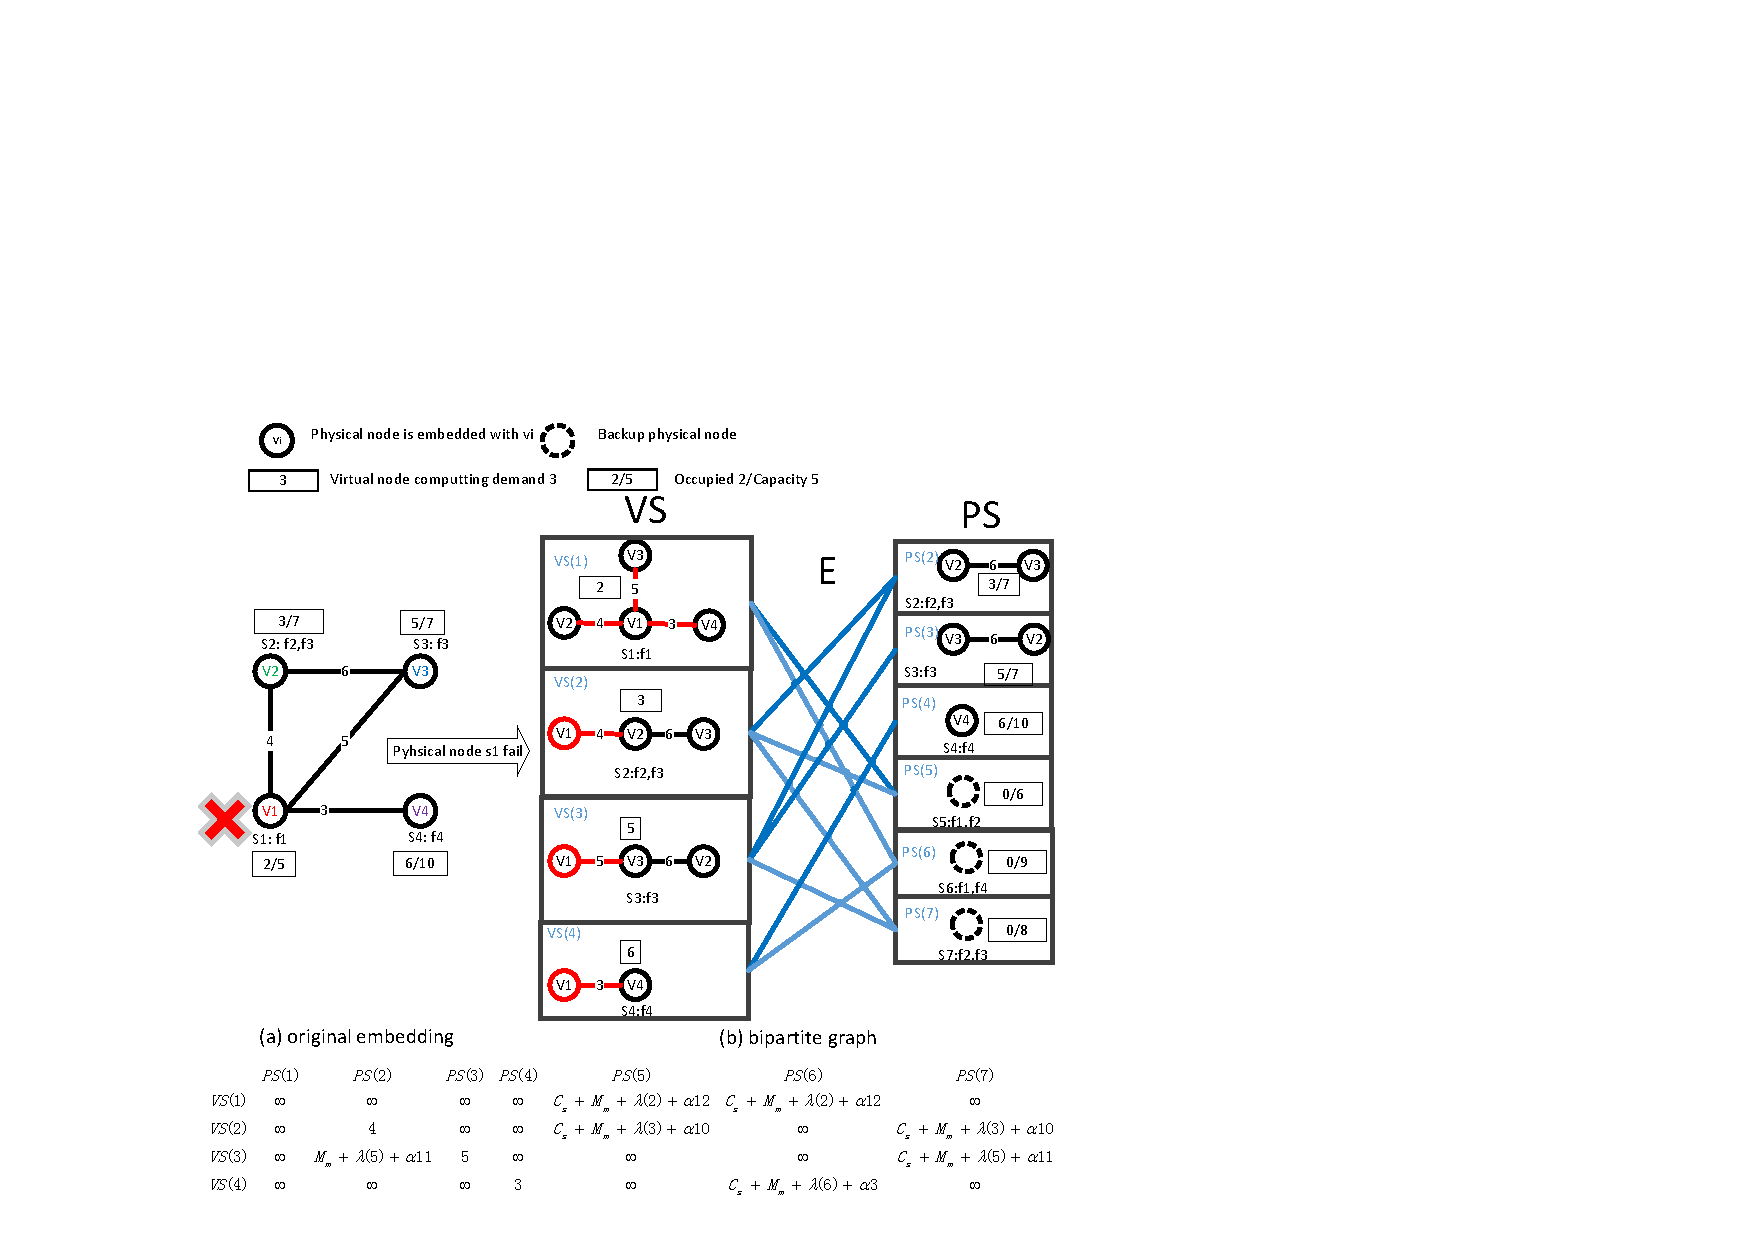
\includegraphics[width=4.5in]{figures/StarRepresentation}\\
  \caption{当物理节点$s_1$ 失效时VirtualStar($v_i$)和PhysicalStar($s_j$)}\label{fig:StarRepresentation}
\end{figure}

\begin{equation*}
\small{
 {\begin{array}{*{20}{c}}
&R_{S_{1}}&R_{S_{2}}&R_{S_3}&R_{S_4}&R_{S_5}&R_{S_6}&R_{S_{7}}\\
{L_{V_1}}&\infty&\infty&\infty&\infty&\fbox{$C_{s}+M_{m}$+(2)+12}&C_{s}+M_{m}+(2)+12&\infty\\
L_{V_2}&\infty&\fbox{4}&\infty&\infty&C_{s}+M_{m}+(3)+10&\infty&C_{s}+M_{m}+(3)+10\\
L_{V_3}&\infty&M_{m}+(5)+11&\fbox{5}&\infty&\infty&\infty&C_{s}+M_{m}+(5)+11\\
L_{V_4}&\infty&\infty&\infty&\fbox{3}&\infty&C_{s}+M_{m}+(6)+3&\infty\\
\end{array}}
}
\label{lab:Node1FaliureAlignmentMatrixNew}
\end{equation*}


对于虚拟节点$v_i$,如果它的虚拟功能不能在具有$f(i) \notin F(i)$ 的物理节点$s_j$ 中执行,则没有边连接在$V_1$ 中的$VirtualStar(v_i)$和在$V_2$中 的$PhysicalStar(s_j)$。为了便于问题表述,我们将边权设为$\infty $。例如,由于$v_1$ 的虚拟功能是$f_1$,所以它不能在物理节点$s_2$ 中执行。因此,与$VirtualStar(v_1)$ 和$PhysicalStar(s_2)$连接时,不添加任何边,我们设置$w(1,2)=\infty$。

对于$VirtualStar(v_2)$,因为$v_2$最初由$s_2$ 持有,但是,当物理节点$s_1$(最初持有$v_1$)失效时,虚拟链路$e_{12}$无法映射到物理网络。我们应该找到一条连接$\phi(v_2)$和$\phi(v_1)$ 满足带宽需求$d_{12}=4$的新路径。因此,边权系数$VirtualStar(v_2)$和$PhysicalStar(s_2)$的值为4。

当节点$s_1$失效时,它直接影响虚拟节点$v_1$。 由于$s_5$ 可以执行虚拟功能$f_1$,我们可以添加一个边来连接$VirtualStar(v_1)$和$PhysicalStar(s_5)$。 然而,在由于$s_5$ 以前没有设置虚拟机,因此还引入了虚拟机的启动成本$C_s$。 因此,链路权重为$C_s$(启动成本)+$M_m$(迁移成本)+3(节点容量成本)+10(带宽成本)。

\subsection{问题定义}
为了提供可生存性的服务,每个虚拟星型图(根虚拟节点和连接根节点及其相邻节点的虚拟链路)都应该映射到物理星型图。假设虚拟网络由n 个虚拟节点组成,因此有n个虚拟星型图。物理网络由m 个物理节点组成,从而构成m 个物理星型图。在等式\ref{eq:indication}中,我们使用二进制位$M_{ij}$ 来表示第i 个虚拟星型图是否映射到第j 物理星型图。

\begin{equation}
{M_{ij}} = \left\{ {\begin{array}{*{20}{c}}
   1 & {map \ v_i \  to  \ s_j}  \\
   0 & {otherwise}  \\
\end{array}} \right.
\label{eq:indication}
\end{equation}

当物理节点发生故障时,为了使备份资源成本最小化,可生存性虚拟网络嵌入问题可以定义如下:
\begin{equation}
\begin{array}{*{20}{c}}
   {\mathop {\min }\limits_{{M_{ij}}} } & {\sum\limits_{i = 1}^n {\sum\limits_{j = 1}^m {{M_{ij}}{w_{ij}}} } }  \\
   {s.t.,} & {\sum\limits_{i = 1}^n {{d_i}{M_{ij}}}  \le {c_j}}  \\
   {} & {\sum\limits_{j = 1}^m {{M_{ij}}}  \le 1}  \\
   {} & {{M_{ij}} = \{ 0,1\} }  \\
\end{array}
\label{eq:problem formulation}
\end{equation}

其中${\sum\limits_{i = 1}^n {\sum\limits_{j = 1}^m {{M_{ij}}{w_{ij}}} } }$ 表示当物理节点失效时将所有虚拟星型图映射到物理星型图的总备份资源成本。在公式\ref{eq:problem formulation} 中,${\sum\limits_{i = 1}^n {{d_i}{M_{ij}}}  \le {c_j}}$是物理节点的容量约束,也就是说,即使允许将多个虚拟节点映射到一个物理节点,总容量需求不应大于物理节点的容量。${\sum\limits_{j = 1}^m {{M_{ij}}}  \le 1}$ 表示一个虚拟星型图只映射到一个物理星型图。

显然,公式\ref{eq:problem formulation}中定义的问题是一个二进制ILP 问题,根据Karp 的21 个NP- 完全问题\cite{karp1975computational},它是一个一般的NP-complete 问题。

\begin{theorem}
公式\ref{eq:problem formulation}是一个NP-complete 问题。
\end{theorem}
\begin{proof}
如果只有一个物理节点m=1,则我们的可生存性虚拟网络嵌入问题可以退化为单背包问题,即NP-完全问题。在实际应用中,m 通常大于1,单背包问题是可生存性虚拟网络嵌入问题的子问题,给出的可行解在多项式时间内很容易验证,根据计算机复杂性领域上的可归约性定理\cite{wood1987theory},得出我们在公式\ref{eq:problem formulation} 中定义问题是NP-complete 的结论。
\end{proof}

\subsection{动态规划方法}
\label{lab:DynamicProgrammingEquation}
虽然求解ILP公式会得到最小成本的可生存性虚拟网络嵌入,但其指数时间复杂度使得这种方法在大型物理网络中嵌入虚拟网络是不可行的。在这一部分中,我提出了一种基于动态规划的算法,该算法仅具有多项式时间复杂度,因此对于实际的网络系统是可行的方法。

为了描述基于动态规划的算法,我们定义了$dp[i][{x_1}][{x_2}] \ldots [{x_m}]$ 表示以最小备份资源代价将前面$i$($0 \le i \le n $)个虚拟星型图放置到物理网络中的m个物理星型图中,其容量限制为$ x_1$, $ x_2$, $\ldots$, $x_m$。

第$i$个虚拟节点可以选择放置在任何一个存活的的物理星型图上。设$\theta (i,j)$ 表示已经将原先$i-1$个虚拟节点最佳放置后再将第$i$ 个虚拟节点放置到第j 个物理节点的备份资源成本。$\theta (i,j)$表示如下:
\begin{equation}
\theta (i,j) = \left\{ {\begin{array}{*{20}{c}}
{dp[i - 1][x_1][{x_2}] \ldots [{x_j} - {d_i}] \ldots [{x_m}] + {w_{ij}}}\\
\infty
\end{array}} \right.\begin{array}{*{20}{c}}
{({x_j} \ge {d_i},{f_i} \in {F_j})}\\
{otherwise}
\end{array}
\label{eq:place i to j}
\end{equation}
在等式\ref{eq:place i to j}中,如果物理节点$x_j$的容量限制大于容量需求$d_i$ 并且在物理节点${f_i} \in {F_j}$能执行虚拟功能$f_i$,则 $\theta (i,j)$ 是已经放置前面i−-1 个最佳虚拟星型图的代价和(即$dp[i-1][{x_1} - {d_i}][{x_2}] \ldots [{x_m}]$) 和将虚拟星型图($v_i$) 映射到物理星型图($s_1$)的成本(即$w_{i1}$)。基于$\theta (i,j)$,$dp[i][{x_1}][{x_2}] \ldots [{x_m}]$可通过以下动态规划函数计算。
\begin{equation}
dp[i][{x_1}][{x_2}] \ldots [{x_m}] = min\{\theta (i,1),\theta (i,2),\ldots,\theta (i,j),\ldots,\theta (i,m)\}
\label{eq:update function}
\end{equation}

基于动态规划的算法如伪码\ref{alg:DPAlg}所示。我们还以如图\ref{fig:DPIllustration}所示中的一个例子来说明该算法。


\begin{figure}[htbp]
\centering
% Requires \usepackage{graphicx}
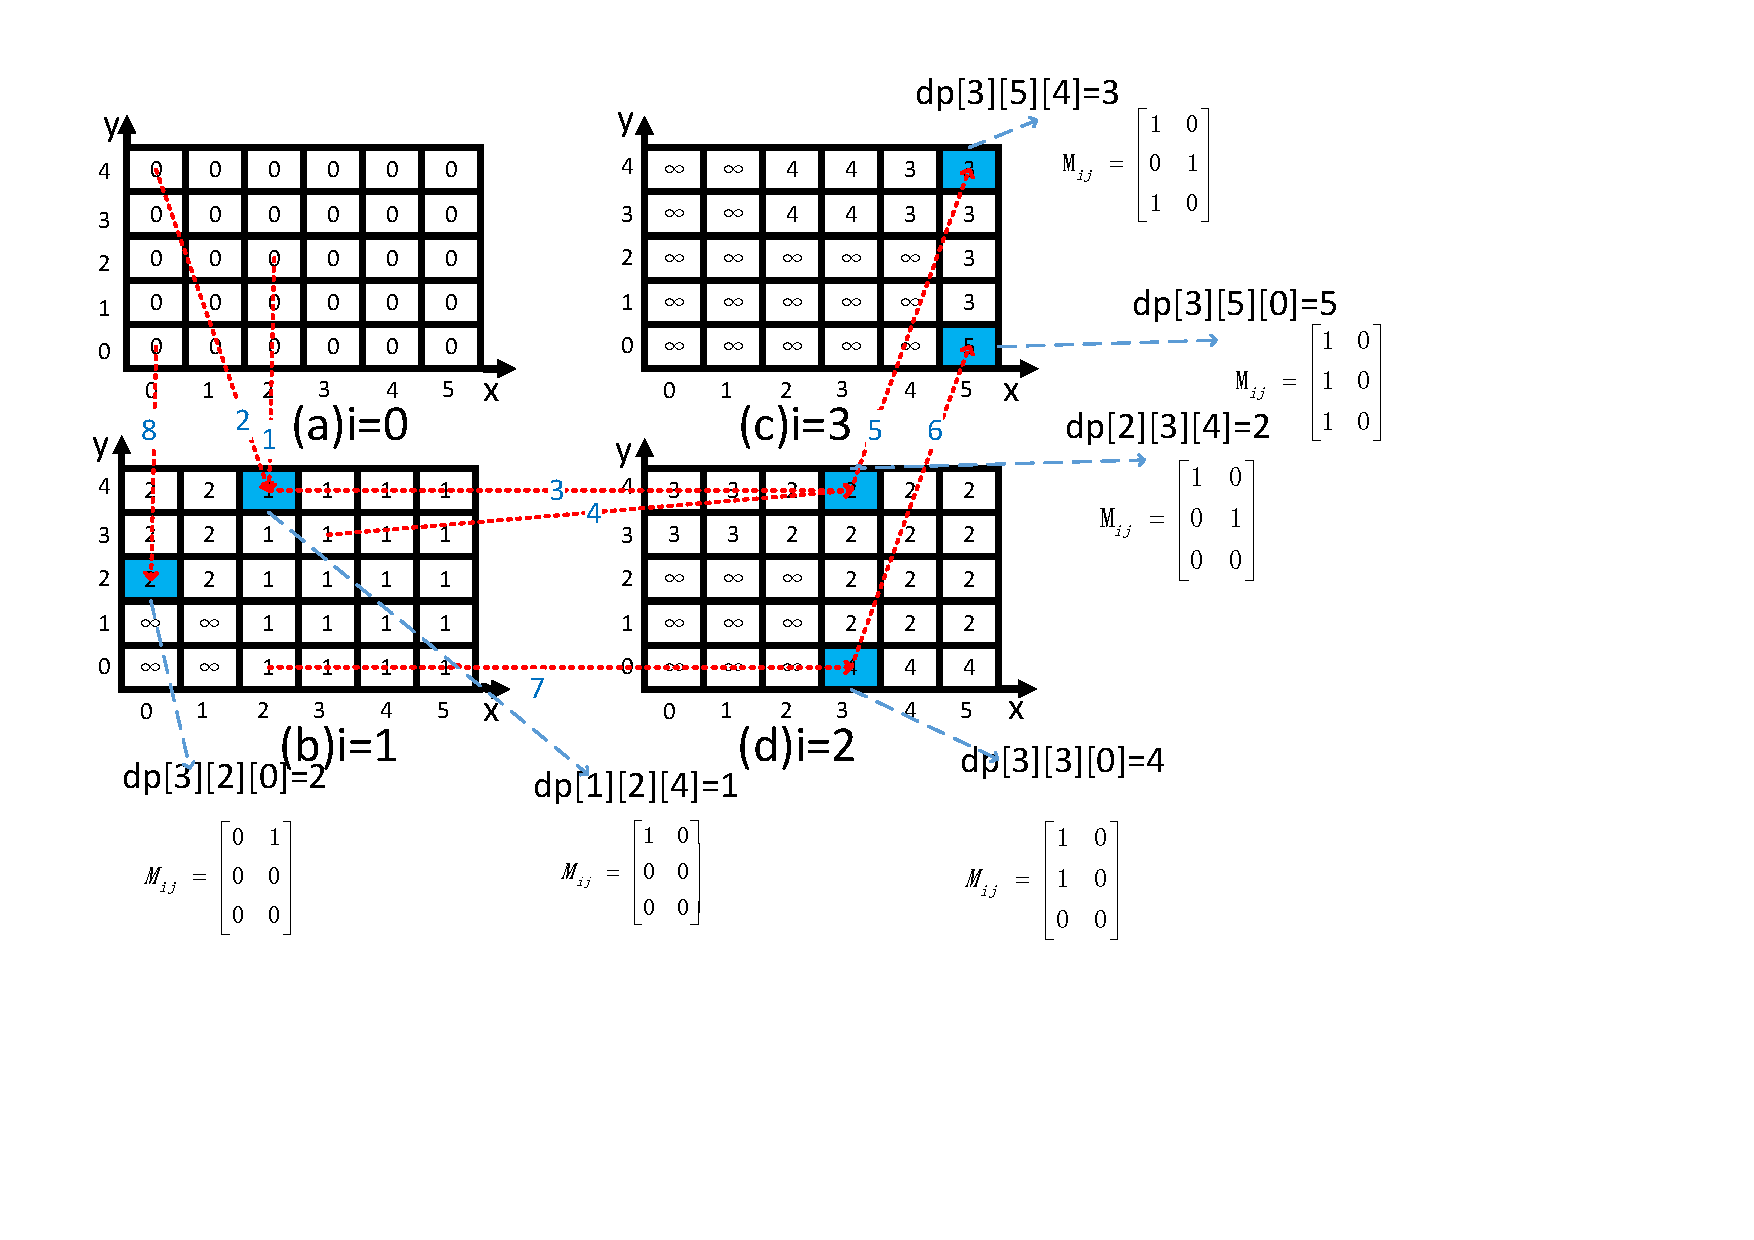
\includegraphics[width=5in]{figures/DPIllustration}\\
  \caption{动态规划方法的演示}\label{fig:DPIllustration}
\end{figure}


\begin{algorithm}[htbp]
\label{alg:DPAlg}
\caption{基于动态规划方法二分星型图匹配算法}
\begin{algorithmic}[1]
\REQUIRE {$dp[i][{x_1}][{x_2}] \ldots [{x_m}]=0(1\leq i \leq n, 0\leq x_1\leq c_1, 0\leq x_2\leq c_2,\ldots, 0\leq x_m\leq c_m)$ 首先被定义成无穷大$\infty$,$dp[0][{x_1}][{x_2}] \ldots [{x_m}]=0(0\leq x_1\leq c_1, 0\leq x_2\leq c_2,\ldots, 0\leq x_m\leq c_m)$, m:物理节点的数量。 $M[{x_1}][{x_2}] \ldots [{x_m}]=\textbf{0}_{n\times m}$ 每个节点的映射矩阵}
\ENSURE {当节点容量为$c_1,c_2,\ldots,c_m$时最小代价的节点映射}
\FORALL{$i$ such that $1\leq i\leq n$ }
\FORALL{$x_1,x_2,\ldots,x_m$ such that $ c_1\geq x_1\geq d_i$, $c_2\geq x_2\geq d_i$,$c_3\geq x_3\geq d_i$,$c_m\geq x_m\geq d_i$}

\STATE {$dp[i][{x_1}][{x_2}] \ldots [{x_m}] = min\{\theta (i,1),\theta (i,2),\ldots,\theta (i,j),\ldots,\theta (i,m)\}$}

\STATE{$j' = \mathop {\arg \min }\limits_j \{\theta (i,1),\theta (i,2),\ldots,\theta (i,j),\ldots,\theta (i,m)\}$, }.
\STATE{$M[{x_1}][{x_2}] \ldots [{x_m}]=M[{x_1}][{x_2}] \ldots[x_{j'}-d_i]\ldots [{x_m}]$}
\STATE{$M[{x_1}][{x_2}] \ldots [{x_m}]_{ij'}=1$}
\ENDFOR
\ENDFOR
\RETURN $dp[i][{c_1}][{c_2}] \ldots [{c_m}]$ and $M[{c_1}][{c_2}] \ldots [{c_m}]$
\end{algorithmic}
\end{algorithm}

在本例中为了清晰地表示,需要将三个虚拟星型图放置到两个可用的物理星型图以实现最小的备份资源成本。物理节点下的可用容量分别为$c_1=5$ 和$c_2=4$。 这三个虚拟星型图的容量需求分别为$d_1=2$,$d_2=1$和 $d_3=2$。 在这些虚拟星型图中需要执行的虚拟功能是$f(1)=f_1$, $f(2)=f_1$, $f(3)=f_2$。这两个物理节点支持的虚拟功能是$F(1)=\{f_1,f_2\}$ 和$F(2)=\{f_1\}$。

如图\ref{fig:DPIllustration}所示, $x$和 $y$ 轴分别表示物理星型图$s_1$ 和$s_2$ 的容量极限。虚拟星型图与物理星型图的连接边的权重$w_{11}=1$, $w_{12}=2$, $w_{21}=3$, $w_{22}=1$, $w_{31}=1$, $w_{32}=\infty$。 最初,在图\ref{fig:DPIllustration}(a) 中,由于没有对任何物理星型图放置虚拟星型图,所有容量限制情况下的备份成本($x_1$=0,1,2,3,4和$x_2$=0,1,2,3,4,5) 都是0。特别是,即使设置了4 和5 的容量限制,dp[0][4][5]=0。如图\ref{fig:DPIllustration}(b)所示,当将容量要求为$d_1=1$ 的第一个虚拟节点$v_1$ 放置到这两个物理节点时,可以在两个物理节点中执行$f_1$。因此,我们有
\begin{equation}
dp[1][{x_1}][{x_2}] = \min \{\theta (1,1),\theta (1,2)\}
\end{equation}

特别是,如果这两个物理节点的容量极限分别为$x_1$=2和$x_2$=0,则$dp[1][2][0]= dp[0][0][0]+w_{11}=2$。如果这两个物理节点的容量极限分别为$x_1$=2和$x_2$=4,则$\theta (1,1)=dp[0][0][2]+w_{11}$和$\theta (1,2)=\infty$,从而$dp[1][2][4]=min\{ dp[0][0][4]+w_{11}, dp[0][2][2]+w_{12} \}=1$。

同样,当将容量要求$d_2=2$的第二个虚拟节点放置到这两个物理节点时,所有容量限制下的成本结果如图\ref{fig:DPIllustration}(d)所示。因为$f_2$ 可以在两个物理节点中执行,因此$v_2$可以放置在两个物理节点中,所以我们有
\begin{equation}
dp[2][{x_1}][{x_2}] = \min \{\theta (2,1),\theta (2,2)\}
\end{equation}


特别是,如果这两个物理节点的容量极限分别为$x_1$=3和$x_2$=4,则$dp[2][3][4]=min\{dp[1][2][4]+w(2,1)$,$dp[1][3][3]+w(2,2)\}=2$。如果这两个物理节点的容量极限分别为$x_1$=3和$x_2$=0,则$dp[2][3][0]=dp[1][2][0]+w(2,1)=4$。

如图\ref{fig:DPIllustration}(d)显示了将容量要求为$d_3=1$的第三个虚拟节点放置到这两个物理节点时的最小资源成本结果。由于$f_3$ 只能在物理节点$s_1$中执行,所以我们有$\theta (3,2)=\infty$。 特别是,如果这两个物理节点的容量极限分别为$x_1$=5 和$x_2$=0,则$dp[3][5][0]=dp[2][3][0]+w(3,1)=4$。由于这两个物理节点的节点能力分别为5 和4,我们得到了$dp[3][5][4]=dp[2][3][4]+w(3,1)=3$,如图\ref{fig:DPIllustration}(d)所示,在dp[3][5][4]=3处得到了最佳位置,节点映射为$v_1\rightarrow s_1, v_2\rightarrow s_2, v_3\rightarrow s_1$。

例如,如图\ref{fig:StarRepresentation}和等式\ref{lab:Node1FaliureAlignmentMatrixNew} 所示,其最小资源成本结果的最优节点映射矩阵如矩阵\ref{eq:StarRepresentationMatrix} 所示。
\begin{equation}
M_{ij}=\left[ {\begin{array}{*{20}{c}}
0&0&0&0&1&0&0\\
1&0&0&0&0&0&0\\
0&1&0&0&0&0&0\\
0&0&1&0&0&0&0
\end{array}} \right]
\label{eq:StarRepresentationMatrix}
\end{equation}
\section{添加备份资源的略}
如果一个节点失败,则在应用算法\ref{alg:DPAlg} 计算最小额外资源后,添加新的物理节点和物理路径来维护网络可生存性服务。如果不包含任何虚拟节点的物理节点在节点失效前就已经添加为备份节点,我们应该将这个物理节点设置为a=1,以指示该物理节点已经容纳过虚拟节点。

由于我们的可生存性虚拟网络嵌入问题是为了在任何一个节点失效时最小化增加的备份资源,而不是给定的一个节点故障,我们应该逐一测试每个节点的故障,并添加足够的备份资源。作为备份资源只需要当节点失效时,备份资源应在不同节点失效时共享。如果我们直接应用公式\ref{eq:edge weight}中定义的成本来计算另一个物理节点失效时的备份资源,因为公式\ref{eq:edge weight}中定义的成本不考虑备份资源共享,则会导致重复添加备份资源的问题。

为了解决这一问题,我们将$M(j)$加入到物理星型结构中,表示在节点失效的情况下迁移到物理节点$s_j$中的虚拟节点集。
\begin{equation}
PhysicalStar(s_j)=(s_j, \phi^{-1}( s_j), c_j, F(j), \phi(N(\phi^{-1}( s_j))), a, M(j))
\end{equation}
由于备份资源应该只添加一次,为了便于表示该约束,我们定义了以下函数。
\begin{equation}
\mu (x) = \left\{ {\begin{array}{*{20}{c}}
   x & {x > 0}  \\
   0 & {x \le 0}  \\
\end{array}} \right.
\end{equation}
当我们测试另一个节点失效时,而不是等式\ref{eq:edge weight} 中定义的代价,我们定义了一个新的代价函数,考虑到不同节点失败时的备份资源共享。

如等式\ref{eq:new edge weight}所示,资源成本是根据两种情况设置的。如果虚拟节点$v_i$最初由物理服务器$s_j$持有,或者$v_i$被迁移到物理服务器,即${{v_i} \in \left( {{\phi ^{ - 1}}({s_j}) \cup M(j)} \right)}$,当它的邻居$v_k \in N(i)$(${\phi \left( k \right) \notin \phi \left( {{\phi ^{ - 1}}({s_j})} \right)}$) 失效时,路径带宽成本为${\sum\limits_{k \in N(i) \cap N(i')} {\mu({d_{ik}} - {d_{i'k}})}  + \sum\limits_{k \in \left( {N(i) - N(i')} \right)} {{d_{ik}}} }$。

\begin{figure*}
  \centering
  % Requires \usepackage{graphicx}
    \begin{equation}
  \footnotesize
w(i,j) = \left\{ {\begin{array}{*{20}{c}}
   {\sum\limits_{k \in N(i) \cap N(i')} {\mu({d_{ik}} - {d_{i'k}})}  + \sum\limits_{k \in \left( {N(i) - N(i')} \right)} {{d_{ik}}} } & {{v_i} \in \left( {{\phi ^{ - 1}}({s_j}) \cup M(j)} \right),{v_{i'}} \in M(j),k \notin \phi \left( {{\phi ^{ - 1}}({s_j})} \right)}  \\
   {\sum\limits_{k \in N(i) \cap N(i')} {\mu({d_{ik}} - {d_{i'k}})}  + \sum\limits_{k \in \left( {N(i) - N(i')} \right)} {{d_{ik}}}  + \lambda f({d_i} - \mathop {\max }\limits_{{v_{i'}}} \left( {{d_{i'}}} \right)) + \beta {M_m} + \theta } & {{v_i} \notin \left( {{\phi ^{ - 1}}({s_j}) \cup M(j)} \right),{v_{i'}} \in M(j)}  \\
\end{array}} \right.
    \label{eq:new edge weight}
    \end{equation}
\end{figure*}

否则,在原先节点失效的测试前这个虚拟节点$v_i$ 没有被一个物理节点持有和迁移到其他物理节点,除了这个带宽成本为${\sum\limits_{k \in N(i) \cap N(i')} {\mu({d_{ik}} - {d_{i'k}})}  + \sum\limits_{k \in \left( {N(i) - N(i')} \right)} {{d_{ik}}} }$,节点的容量成本为${\lambda * \mu({d_i} - \mathop {\max }\limits_{{v_{i'}}} \left( {{d_{i'}}} \right))}$,虚拟服务器迁移的代价为${\beta * {M_m}}$ 和 $\theta$是从映射虚拟星型图$v_i$ 到物理星型图$s_j$ 的代价。如${\mu({d_i} - \mathop {\max }\limits_{{v_{i'}}} \left( {{d_{i'}}} \right))}$ 而言,如果备份容量已分配的最大值${\mathop {\max }\limits_{{v_{i'}}} \left( {{d_{i'}}} \right)}$大于当前映射(即$d_i$),不需要任何资源,否则,备份资源还缺少${{d_i} - \mathop {\max }\limits_{{v_{i'}}} \left( {{d_{i'}}} \right)}$。

对于$VirtualStar(v_2)$,由于$v_3$最初由$s_3$ 持有,但是当物理节点$s_1$ 失效时,我们可以将虚拟节点$v_3$迁移到物理节点$s_2$,因为$s_2$ 是以前已经安装过虚拟机,因此,成本包括虚拟链路带宽成本$11$,节点容量成本5,虚拟机迁移成本$M_m$。

基于节\ref{lab:DynamicProgrammingEquation}的方法,在物理节点$s_1$失效时得到最佳节点映射:$v_1 \rightarrow s_5$, $v_2 \rightarrow s_2$, $v_3 \rightarrow s_3$, $v_4 \rightarrow s_4$。 物理节点$s_5$ 开始为虚拟节点$v_1$ 建立和应用2个节点计算资源,并分别找到带宽约束为4、5、3 的对应的虚拟链路$(v_1,v_2),(v_1,v_3),(v_1,v_4)$ 的三个物理路径。

如图\ref{fig:StarRepresentationNode2}展示了二分图的一个例子,物理节点$s_2$ 在物理节点$s_1$ 失效之后再失效。这个二分图的边权矩阵可以用矩阵\ref{lab:Node2FaliureAlignmentMatrixNew}表示。
\begin{equation*}
\small{
 {\begin{array}{*{20}{c}}
&R_{S_{1}}&R_{S_{2}}&R_{S_3}&R_{S_4}&R_{S_5}&R_{S_6}&R_{S_{7}}\\
{L_{V_1}}&\fbox{4}&\infty&\infty&\infty&M_{m}&C_{s}+M_{m}+(2)+12&\infty\\
L_{V_2}&\infty&\infty&\infty&\infty&\fbox{$M_{m}$+(1)+5}&\infty&C_{s}+M_{m}+(3)+10\\
L_{V_3}&\infty&\infty&\fbox{5}&\infty&\infty&\infty&C_{s}+M_{m}+(5)+11\\
L_{V_4}&\infty&\infty&\infty&\fbox{3}&\infty&C_{s}+M_{m}+(6)+3&\infty\\
\end{array}}
}
\label{lab:Node2FaliureAlignmentMatrixNew}
\end{equation*}

\begin{figure}[htbp]
\centering
% Requires \usepackage{graphicx}
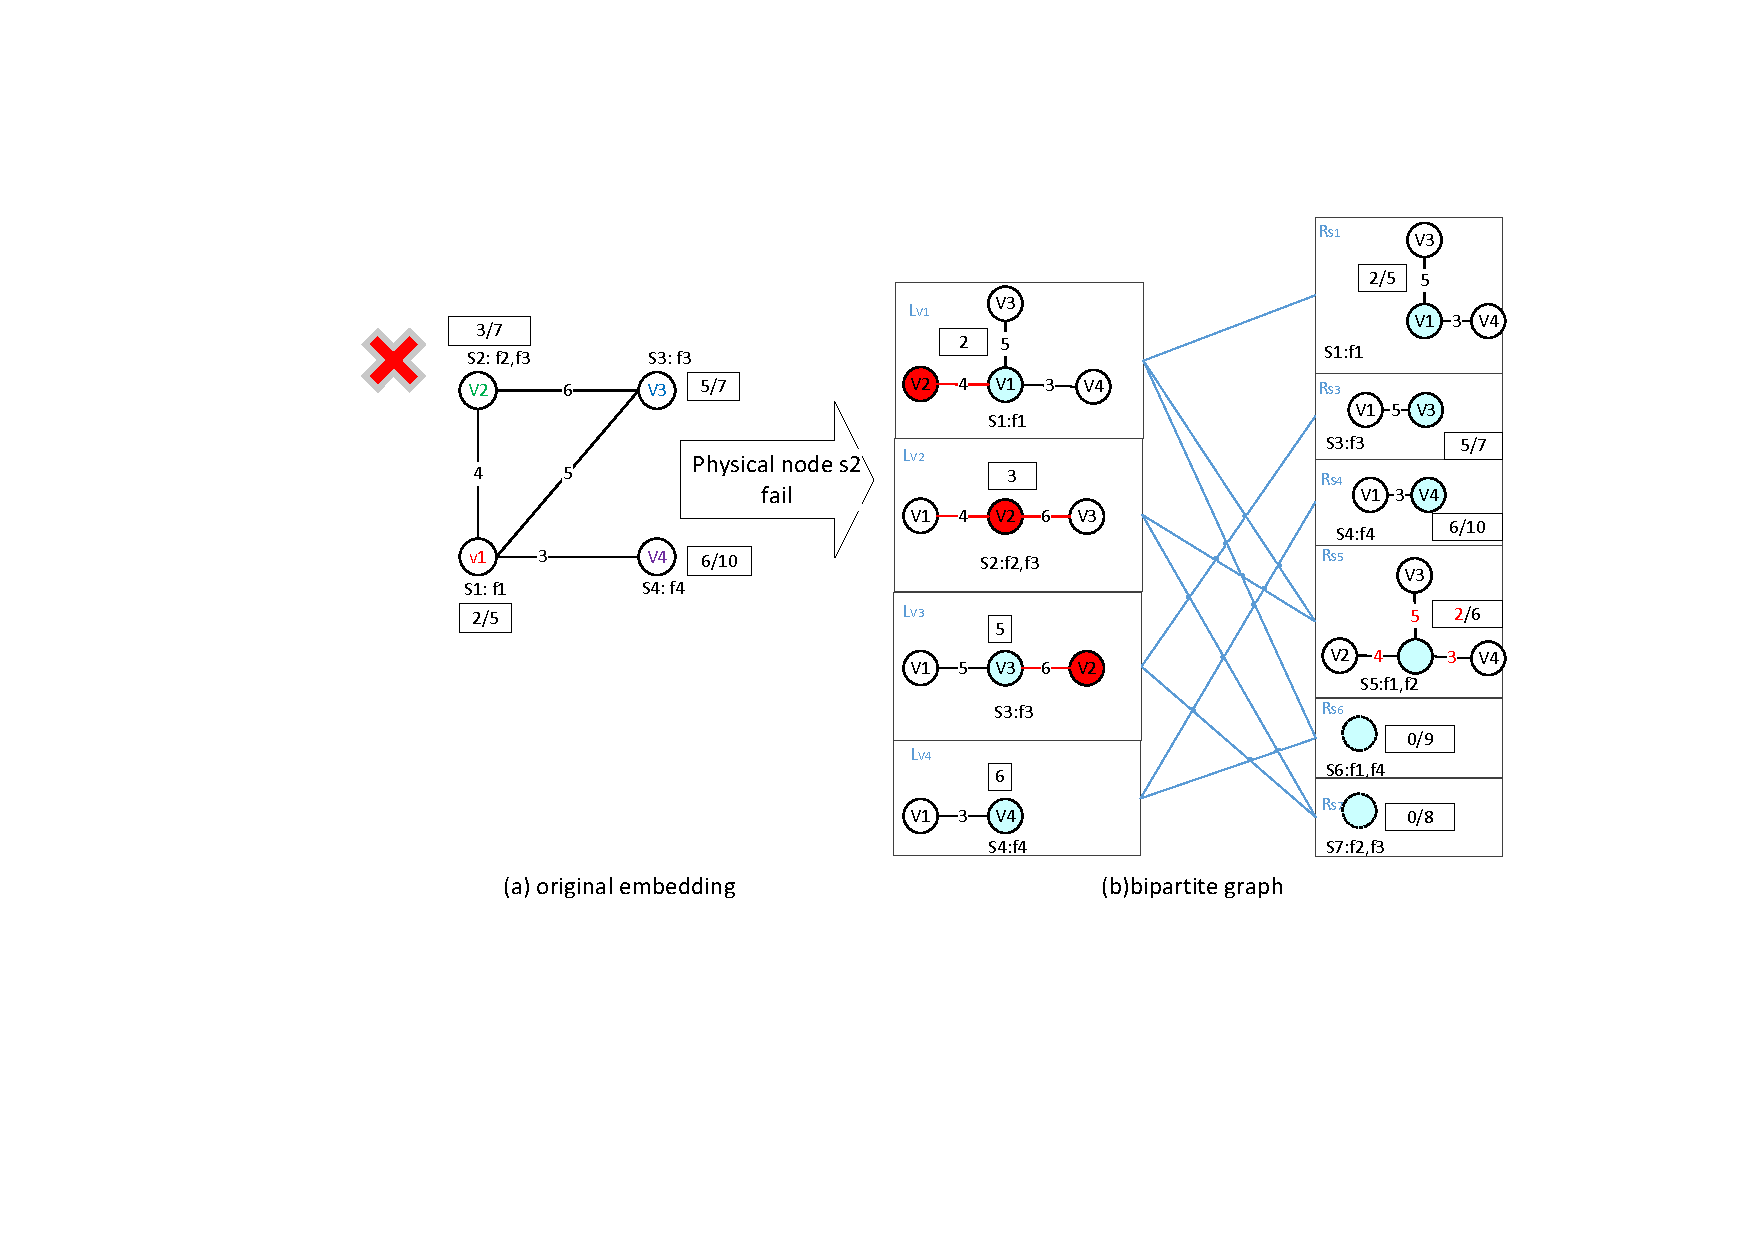
\includegraphics[width=4.5in]{figures/StarRepresentationNode2}\\
  \caption{当物理节点$s_2$ 失效时VirtualStar($v_i$)和PhysicalStar($s_j$)}\label{fig:StarRepresentationNode2}
\end{figure}

\section{多节点故障情形}
\label{sec:multiplePhysicalNodeFailure}
如图\ref{fig:StarRepresentationTwoFailure}所示给出了当物理节点$s_1$和$s_2$ 同时失效时星型二分图的一个例子。这种二分图的边权矩阵可以用矩阵\ref{lab:Node1Node2FaliureAlignmentMatrixNewTwoFailure}表示。
\begin{figure}[htbp]
\centering
% Requires \usepackage{graphicx}
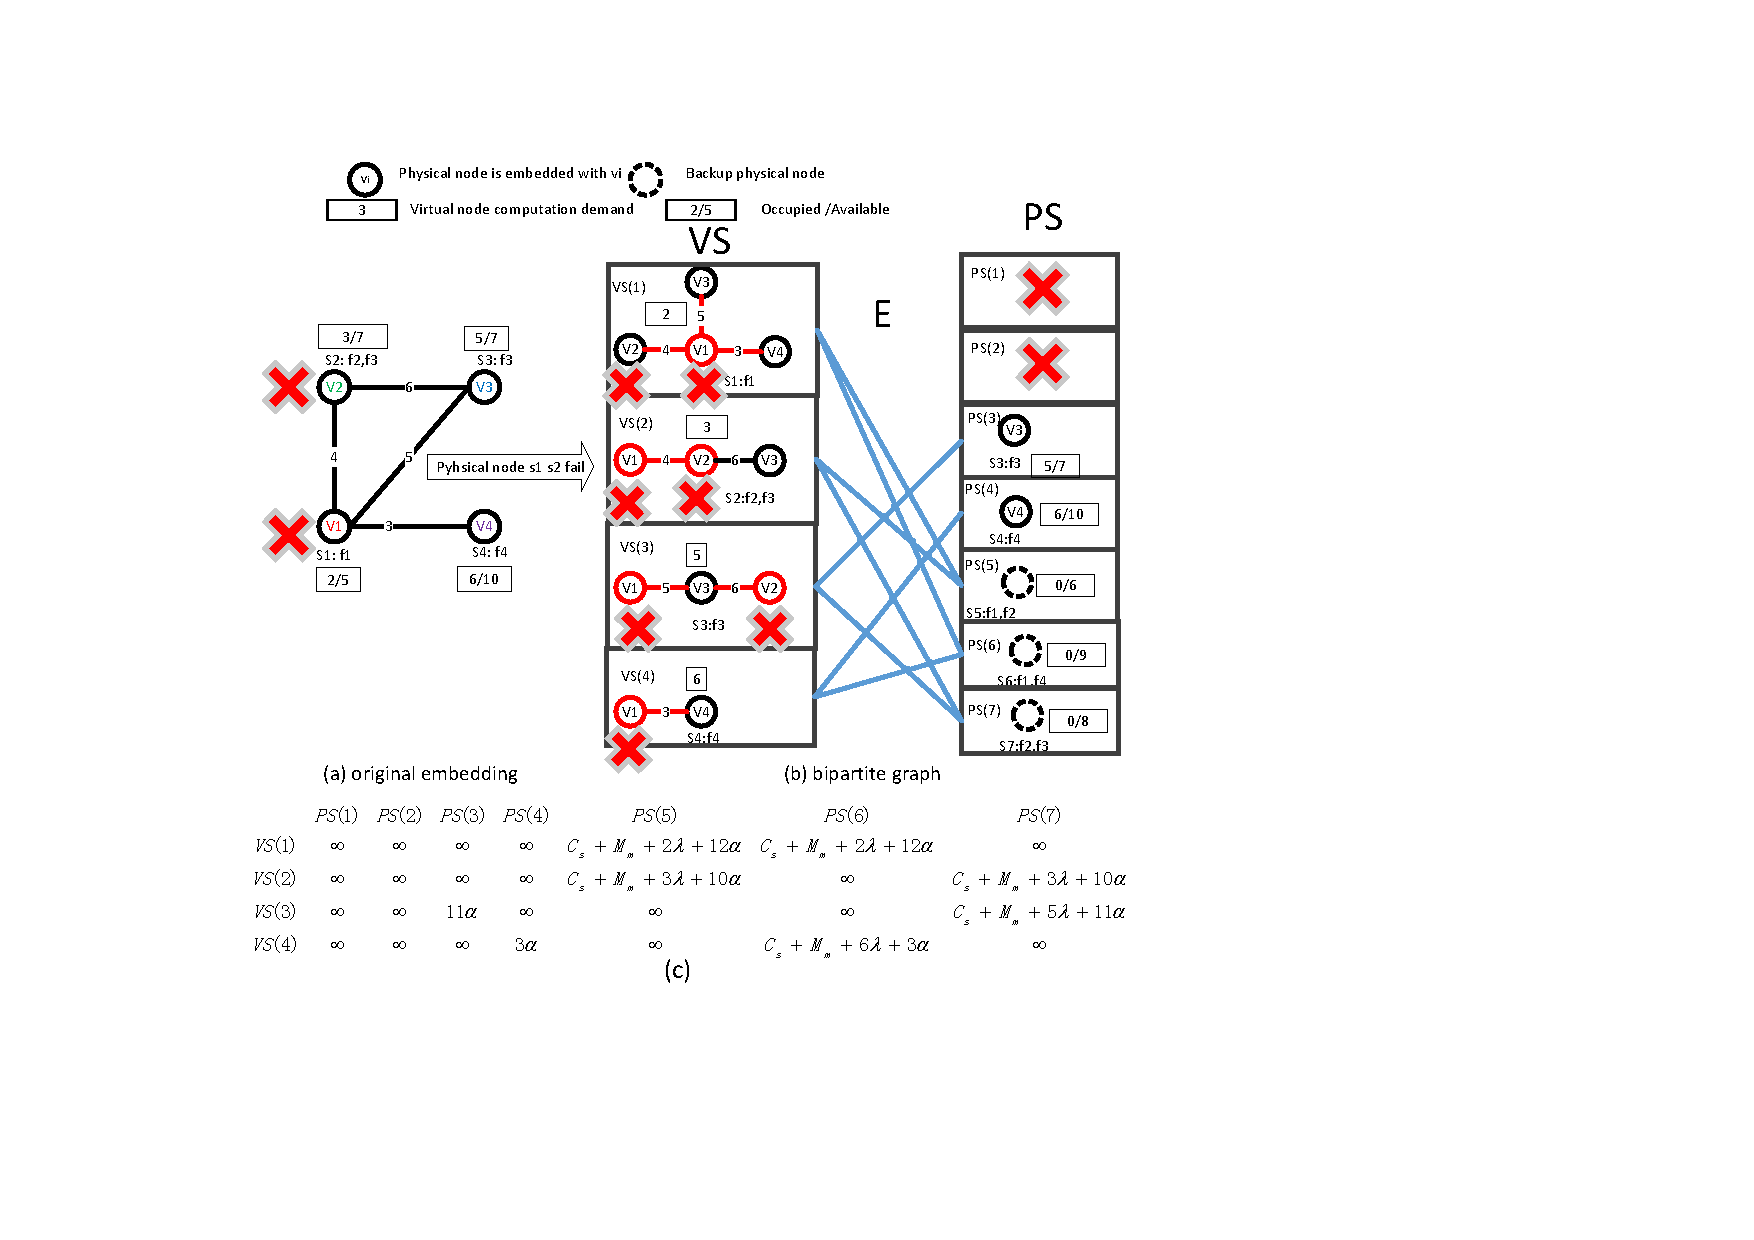
\includegraphics[width=3.8in]{figures/StarRepresentationTwoFailure}\\
  \caption{当物理节点$s_1$和$s_2$同时失效时VirtualStar($v_i$)和PhysicalStar($s_j$)}\label{fig:StarRepresentationTwoFailure}
\end{figure}
\begin{equation*}
\small{
 {\begin{array}{*{20}{c}}
&R_{S_1}&R_{S_2}&R_{S_3}&R_{S_4}&R_{S_5}&R_{S_6}&R_{S_{7}}\\
{L_{V_1}}&\infty&\infty&\infty&\infty&\fbox{$C_{s}+M_{m}$+(2)+12}&C_{s}++M_{m}+(2)+12&\infty\\
L_{V_2}&\infty&\infty&\infty&\infty&C_{s}+M_{m}+(3)+10&\infty&\fbox{$C_{s}+M_{m}+(3)+10$}\\
L_{V_3}&\infty&\infty&\fbox{5}&\infty&\infty&\infty&C_{s}+M_{m}+(5)+11\\
L_{V_4}&\infty&\infty&\infty&\fbox{3}&\infty&C_{s}+M_{m}+(6)+3&\infty\\
\end{array}}
}
\label{lab:Node1Node2FaliureAlignmentMatrixNewTwoFailure}
\end{equation*}
\section{完整算法步骤}
在这一部分中,我们首先给出了SeVN图的增广资源分配过程。下面将详述更多细节。

此外,对于节点嵌入和虚拟链路嵌入,由于单个节点失效时并不是所有的虚拟链路或它们的带宽都会同时使用,所以如果将虚拟链路嵌入在同一底层物理链路上,则一些虚拟链路可以共享底层物理资源。减少总底层物理带宽所需。简单地说,底层物理链路对应不同虚拟网络节点失效时可生存性请求的备份带宽可以相互共享。
\subsection{将增广的备份资源嵌入到底层网络中}

从节\ref{lab:DynamicProgrammingEquation}中,我得到了节点$v_i$失效的节点映射和链路映射关系,和计算出每个节点需要重新分配的计算量,以及每个链路在底层物理网络SN 中应该重新分配的带宽,如图\ref{fig:AugmentResource}所示。分别在物理节点$s_1,s_2,s_3,s_4,s_5,s_6,s_7$中增加计算资源0、2、0、0、3、6、0。查找带宽分别为1,4,6,3,6,6与物理路径$p_{s_1s_2},p_{s_1s_3},p_{s_1s_5},p_{s_1s_6},p_{s_2s_5}$对应的五条路径。尽管虚拟网络嵌入算法很多,但相对于我们的算法,节点映射阶段已经完成,接下来的步骤描述了链路映射阶段。我们使用标准最短路径算法Dijkstra 算法\cite{skiena1990dijkstra}来请求底层物理节点的扩展路径,并为这种虚拟网络生存的请求的部分带宽重新分配给这些路径。一些研究\cite{yu2008rethinking}集中在路径嵌入和路径分割嵌入,以实现高的链路利用率、链路压力和其他目标,但本文没有重点讨论链路映射问题。

\begin{figure}[htbp]
\centering
\begin{minipage}{0.4\textwidth}
\centering
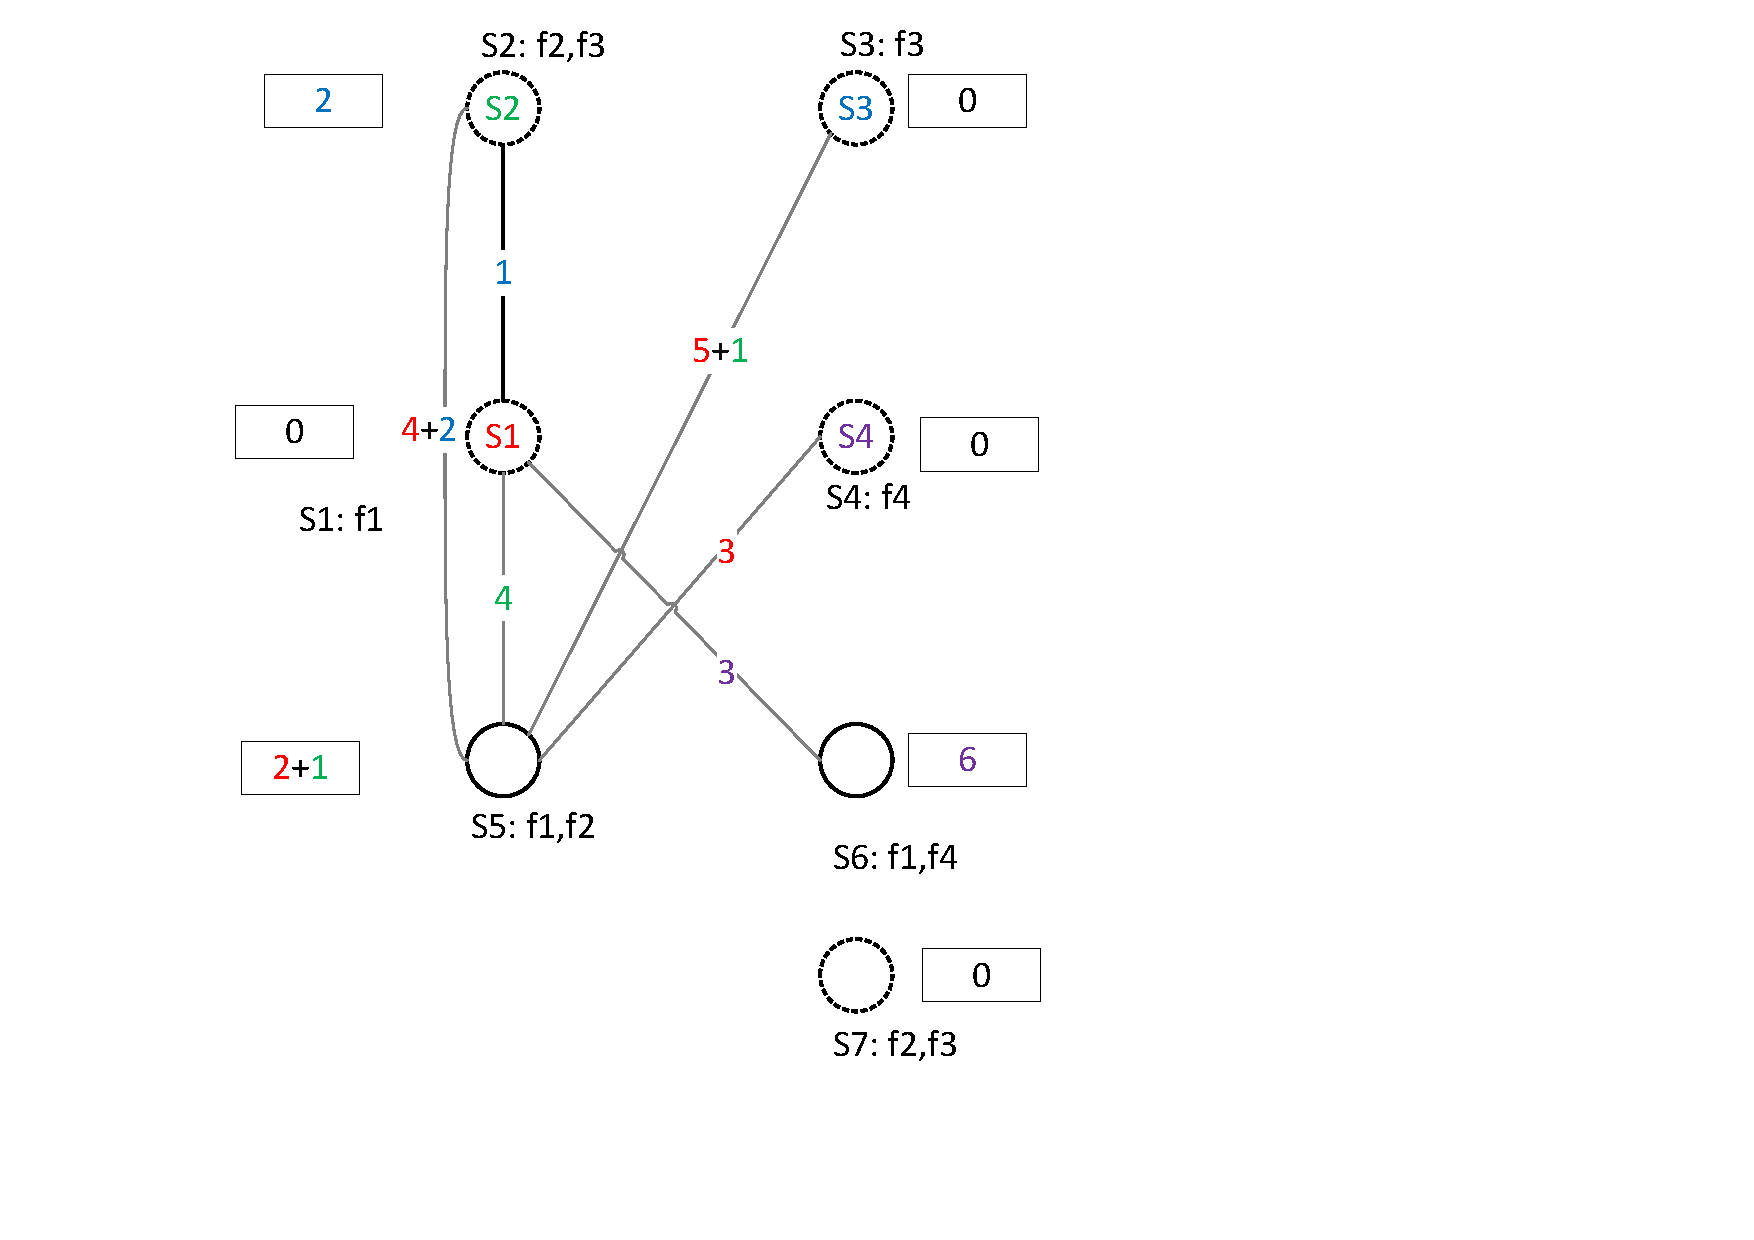
\includegraphics[width=\textwidth]{figures/AugmentResource}
\caption{增广的备份资源图}\label{fig:AugmentResource}
\end{minipage}
\begin{minipage}{0.4\textwidth}
\centering
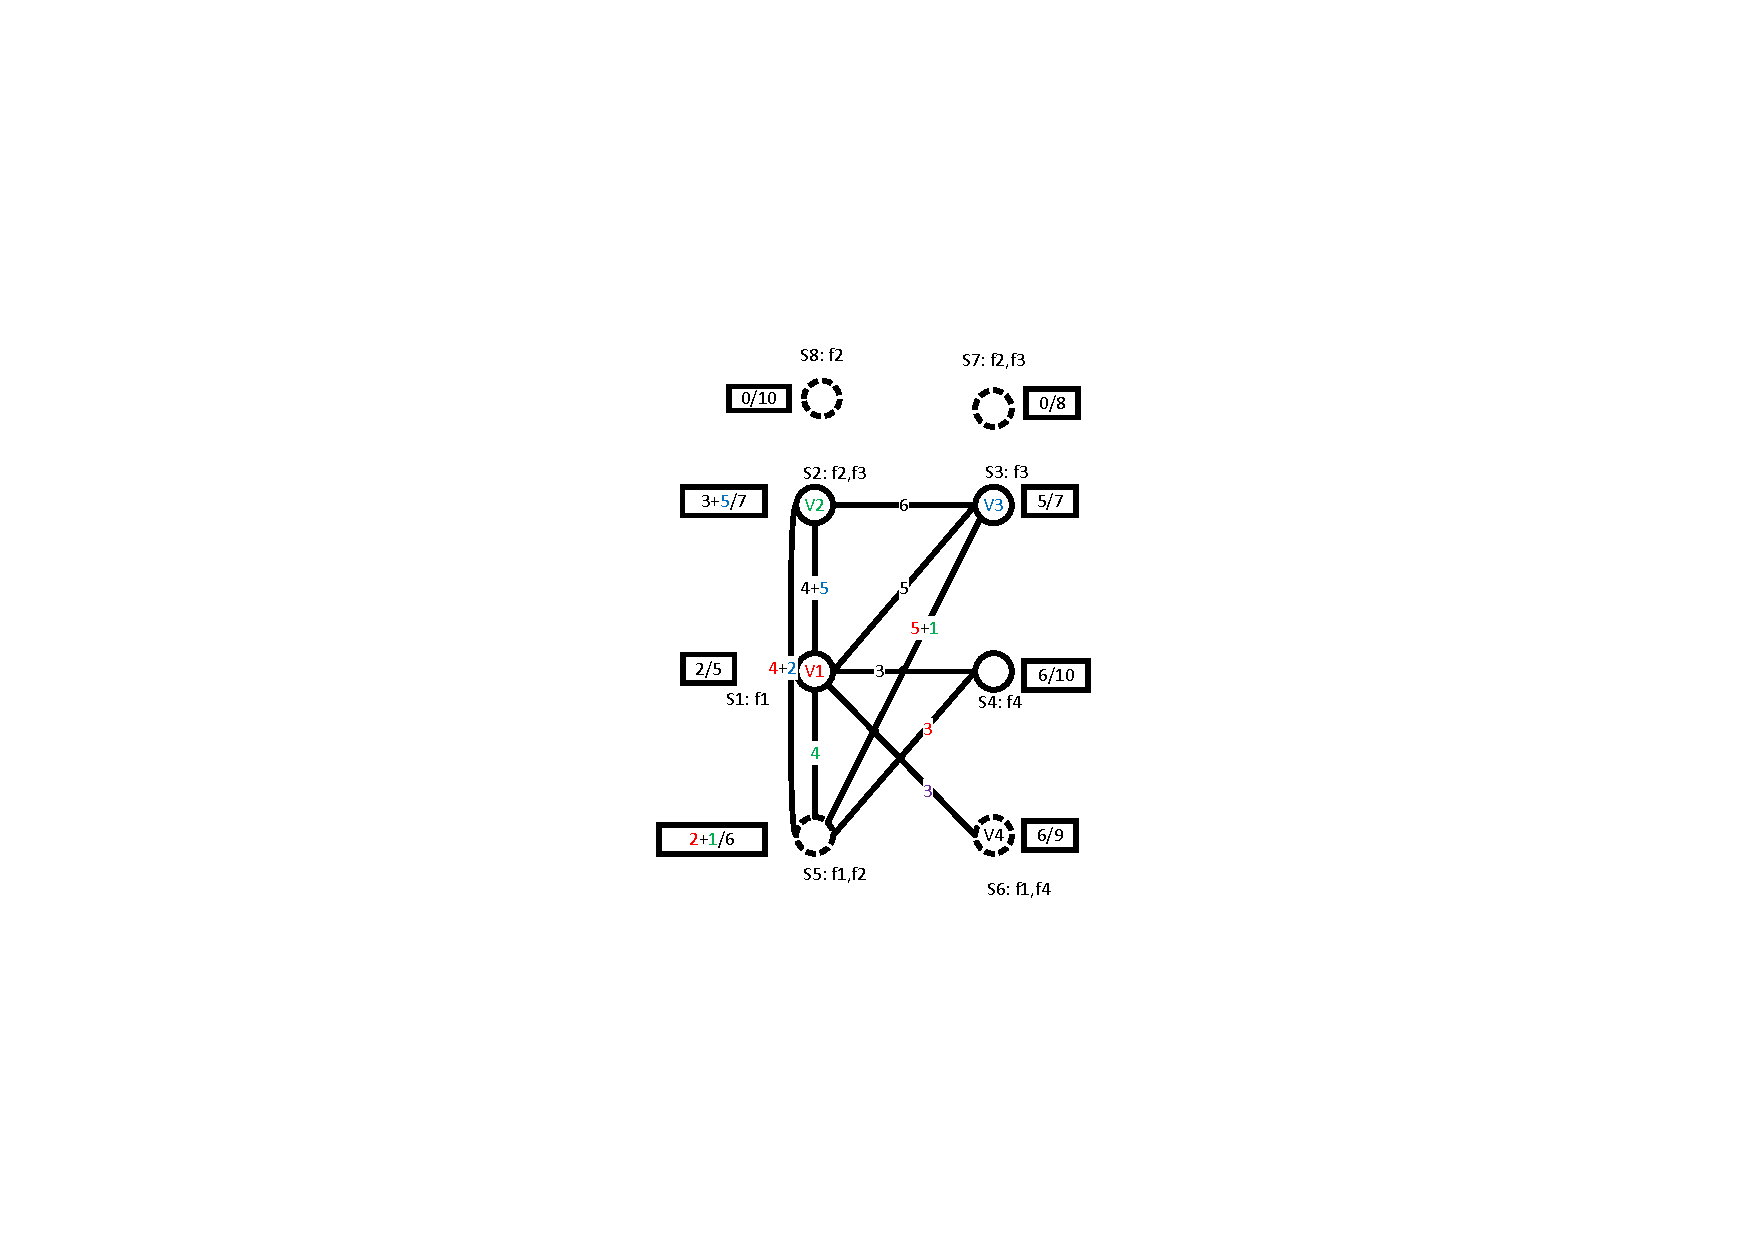
\includegraphics[width=\textwidth]{figures/Node4Failure}
\caption{节点$s_4$失效实例}\label{fig:Node4Failure}
\end{minipage}\vspace{\baselineskip}
\end{figure}

%\begin{figure}[htbp]
%  \centering
%  % Requires \usepackage{graphicx}
%  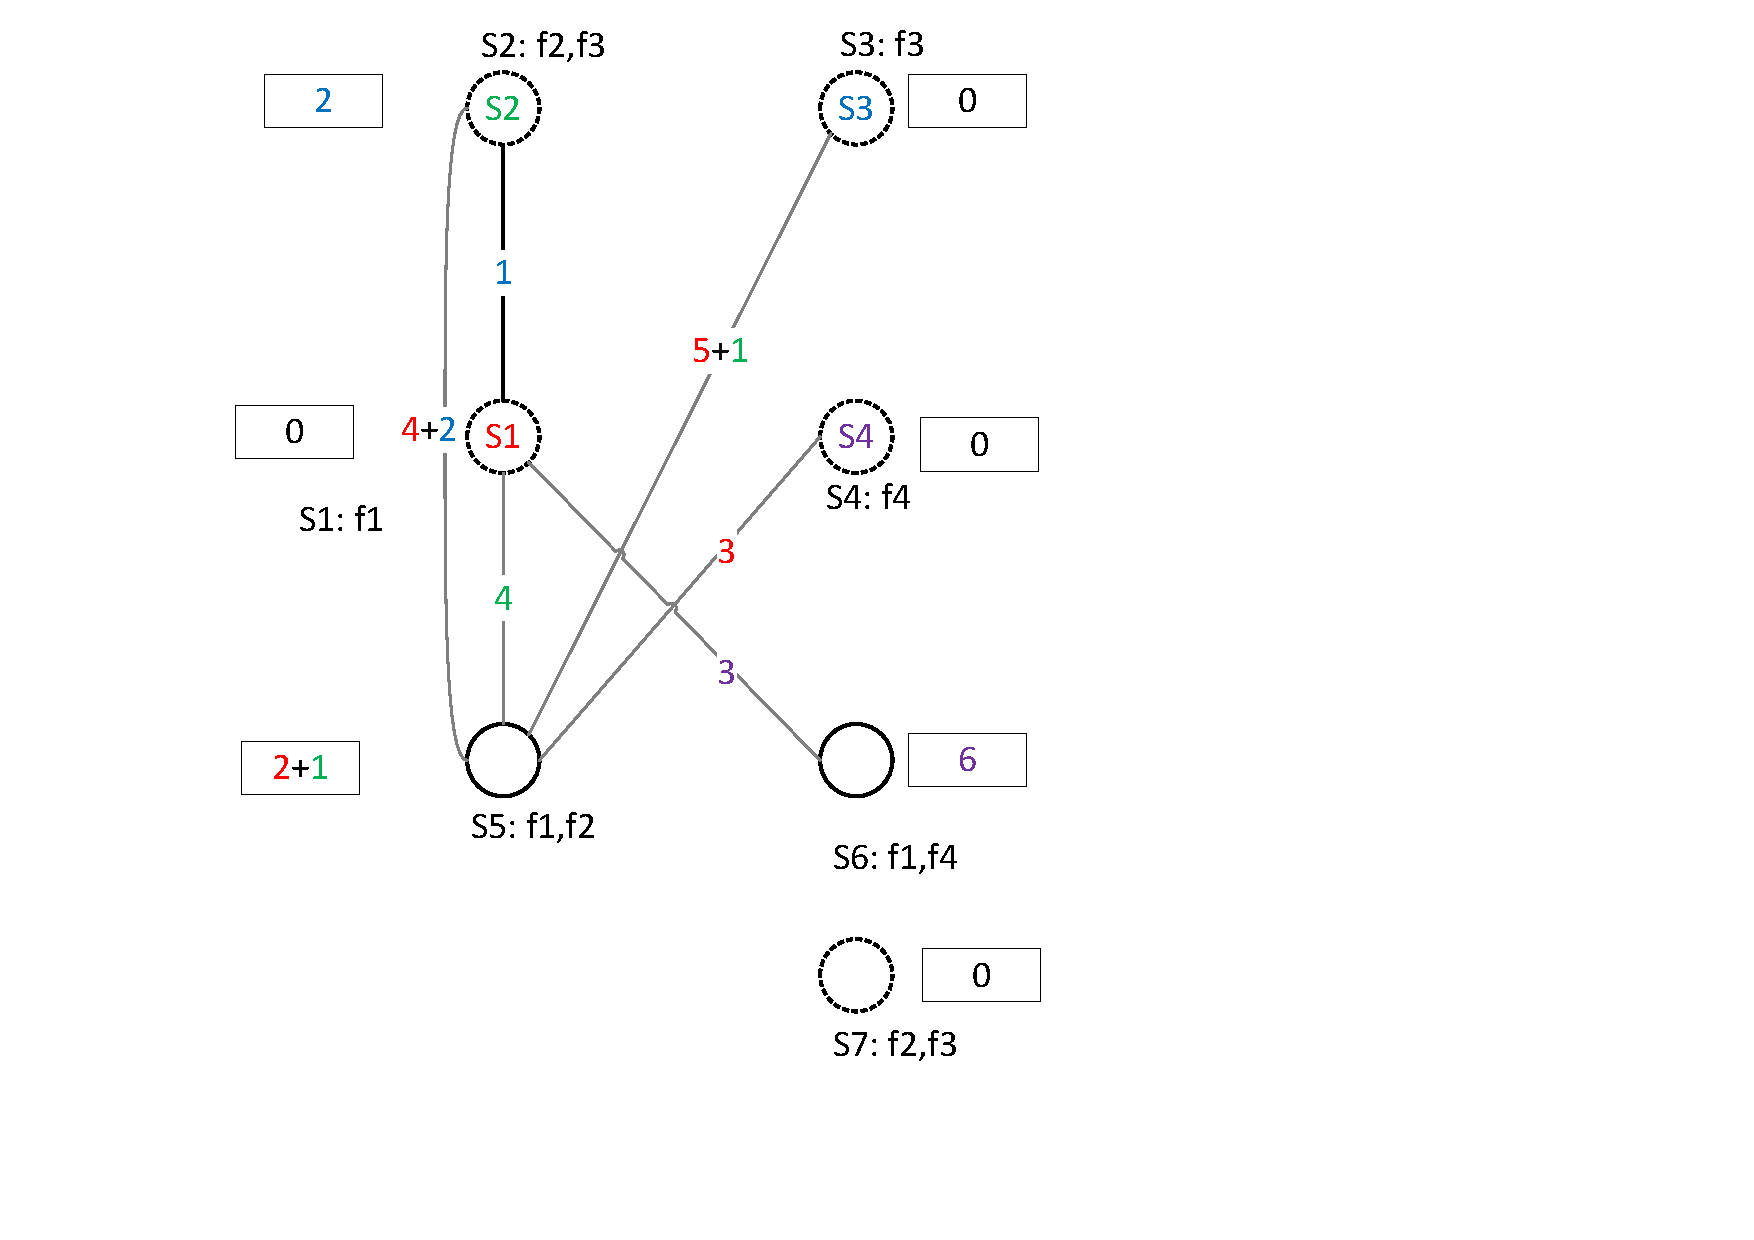
\includegraphics[width=3.0in]{figures/AugmentResource}\\
%  \caption{增广的备份资源图}\label{fig:AugmentResource}
%\end{figure}
最后,迭代的重复图分解过程和多背包问题求解过程,处理每个嵌入虚拟节点的物理节点失效情况,重新构造增强图,以保证虚拟网络的生存请求。如图\ref{fig:Node4Failure}所示,连续使用不同颜色标记SeVN的部分增广资源并且连续显示每个节点故障。值得注意的是,部分增广资源的每一步都是基于前一步的资源增强。
%\begin{figure}[htbp]
%\centering
%% Requires \usepackage{graphicx}
%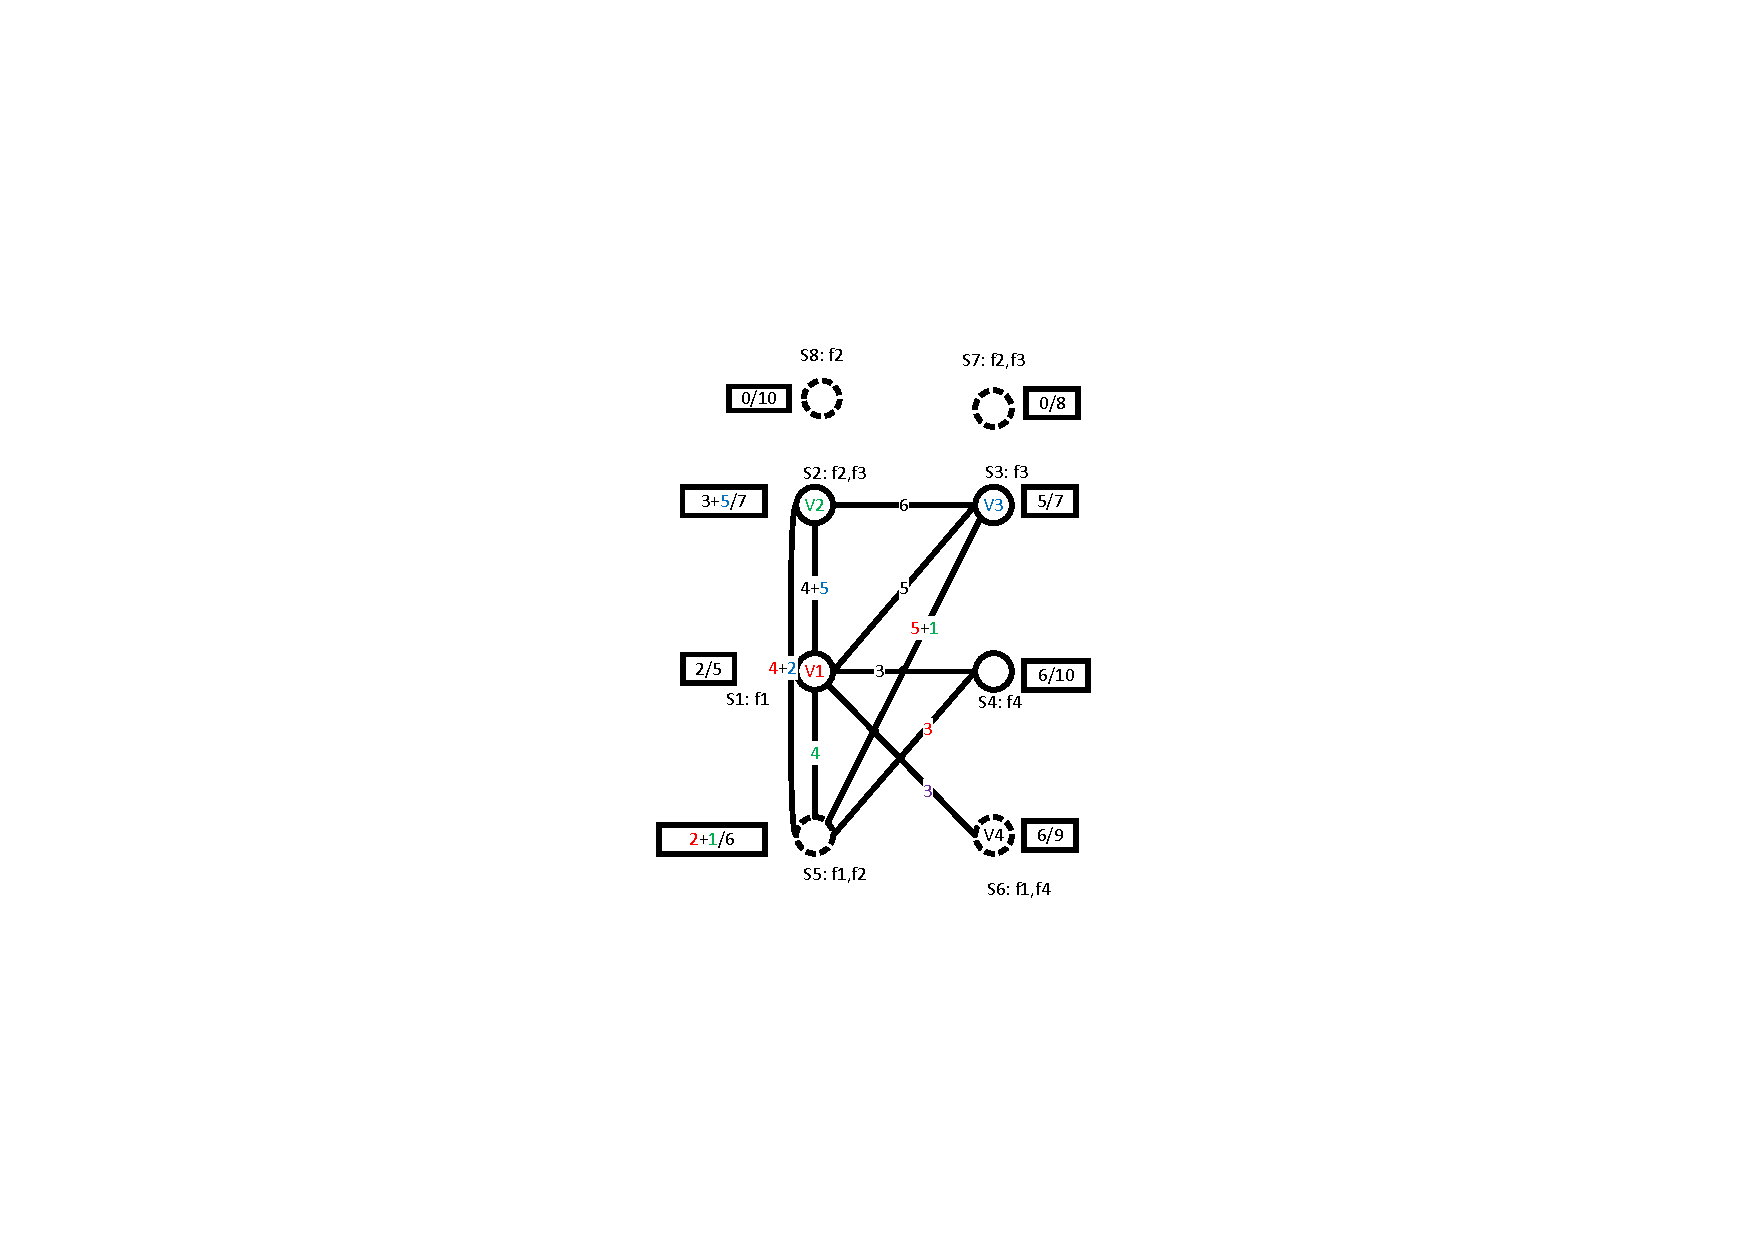
\includegraphics[width=3.0in]{figures/Node4Failure}\\
%  \caption{节点$s_4$失效实例}\label{fig:Node4Failure}
%\end{figure}
\subsection{算法步骤}
在本节中,我们描述了SeVN问题完整的算法步骤,如伪码\ref{alg:SeVNAlg} 所示
\begin{algorithm}
\label{alg:SeVNAlg}
\caption{可生存性虚拟网络嵌入算法}
\begin{algorithmic}[1]
\REQUIRE $G (V,E)$:虚拟网络请求; $G (S,L)$:物理网络。
\ENSURE 生成SeVN并增加资源将SeVN嵌入到底层物理网络中。
\STATE 将虚拟网络$G^V$ 嵌入\cite{liu2011completing}到底层网络$G^S$中
\STATE 从与此VN嵌入请求对应的SN中提取嵌入的虚拟网络eVN$G\left( {\hat S,\hat L} \right)$
%\STATE AllMinimumCycle($G(V,E)$)
\FORALL{$v_i$ 并且 $v_i\in G\left( {\hat S,\hat L} \right)$}
\STATE  从图 $G\left( {\hat S,\hat L} \right)$中分解 eVN $G\left( {\hat S,\hat L} \right)$ 成两个星型结构集 $VirtualStar(v_i)$ 和 $PhysicalStar(s_j)$
\STATE 构建items根据星型结构集 $VirtualStar(v_i)$.
\STATE 构建knapsacks根据星型结构集$PhysicalStar(s_j)$
\STATE 构建边权值矩阵\ref{eq:new edge weight}.
\STATE 根据节\ref{lab:DynamicProgrammingEquation}所描述的动态规划方法解决多背包问题
\STATE 添加新节点,连接新的边,重新分配节点计算资源和链路的带宽资源到$G\left( {\hat S,\hat L} \right)$中构建新的$G\left( {\hat S,\hat L} \right)$
\ENDFOR
\STATE 从 $G\left( {\hat S,\hat L} \right)$中嵌入增广资源到物理网络$G(S,L)$
\end{algorithmic}
\end{algorithm}
\section{时间复杂度}
对SeVN请求问题分析,该问题是优化领域中的二次规划问题,而SeVN问题解的实质是一系列排列矩阵,决定了每个节点失效后的迁移重分配过程。虚拟网络$|V|$节点全部都依次失效,每个节点的迭代时间复杂度为$O[|V|*|S|*\prod_{i=1}^{|S|}c^i]$。 因此,其总体计算复杂度为$O[|V|*|S|*|V|*\prod_{i=1}^{|S|}c^i]$,其中$|V|$为失效节点数。


\section{仿真配置与评价指标}
首先描述了仿真配置,然后给出了评价指标。
\subsection{实验环境}
对于任何VN请求,VN节点的数目是由3到10之间的均匀分布随机得到的,每一对虚拟节点都是以概率0.5 随机连接的。VN节点的计算需求从1到5 之间随机分布,并且VN 上的带宽从1到10之间随机分布。

VN请求的到达服从泊松过程(平均每1时间单位请求15次)。请求的持续时间服从指数分布,平均100个时间单位,高的请求率和较长的租用时间保证了物理基础设施的高利用率。

根据\cite{yu2010survivable},即$\lambda/\alpha=\RelativeCostbetweenComputingBandwidth$,节点的计算资源与链路的带宽资源的相对成本为3。 使用的SN 拓扑是SNDlib拓扑数据\cite{orlowski2010sndlib}如表\ref{tab:SNDlibTopo}所示。 底层物理节点(链路)的计算(带宽)资源都是整数的。分别分布在10至20(50 至100)之间。为了对设备节点失效场景进行建模,我们选择了底层物理网络中的所有底层物理设备节点逐个失效,并统计了每$\SubStrateFacilityNodeFailDuration$个时间单元的迁移频率。
\begin{table}[htb]
\centering
\caption{SNDlib拓扑数据}\label{tab:SNDlibTopo}
\begin{tabular}{|c|c|c|}
  \hline
  % after \\: \hline or \cline{col1-col2} \cline{col3-col4} ...
  数据集 & 节点 & 链路 \\
  \hline
  cost266& 37& 57\\
  geant& 22& 36\\
  germany50& 50& 88\\
  giul39& 39& 172\\
  janos-us-ca& 39& 122\\
  janos-us& 26& 84\\
  nobel-eu& 28& 41\\
  norway& 27& 51\\
  pioro40& 40& 89\\
  ta1& 24& 55\\
  ta2& 65& 108\\
  zib54& 54& 81\\
  \hline

\end{tabular}
\end{table}

为了进行性能比较,除了我提出的方案(由$\MyAlgorithmMethodAbrreviation$命名)之外,我还实现了其他可生存的算法$\SecondAlgorithmMethodAbrreviation$  \cite{yeow2010designing}如下:
\begin{enumerate}
  \item $\SecondAlgorithmMethodAbrreviation$ :算法将备份节点与关键节点之间、备份节点与备份节点之间的连接起来,而不连接关键节点与关键节点之间,关键节点表示嵌入物理节点中的虚拟节点,备份节点表示的增广节点。
  \item $\FouthAlgorithmMethodAbrreviation$:当与虚拟节点映射的底层物理上的每个节点失效时,一种简单的方法是增加一个新的物理节点,用于迁移失败的虚拟节点,并将新的链路与失败的物理节点连接起来。
\end{enumerate}

此外,我们还与虚拟网络嵌入算法\cite{liu2011completing}进行了比较,后者是虚拟网络请求第一次到达时的嵌入方法,其中VN没有可生存性要求,虚拟网络嵌入算法请求(标记为$\ThirdAlgorithmMethodAbrreviation$)作为衡量可生存性所消耗的扩展资源量的标准算法,在实验评估图中标记为“algorithm shared”或者“algorithm Noshared”。 我们假设当一个虚拟网络嵌入到底层物理网络中时,对于$\ThirdAlgorithmMethodAbrreviation$算法来说,就需要有成功的可生存性保证。

基于底层物理网络的资源,无论是共享的还是非共享的(专用的)\cite{lu2006efficient},我们在资源分配模式上独立地实现了这两种情况。每个虚拟网络请求的相应的备份需求相应的底层物理资源可以相互共享,并具有可生存性保证。“专用的”意味着对每个虚拟网络是一个完整的备份网络,备份资源完全用到虚拟网络中,相互独立。但是这是资源效率低下的,因为对于每个获得嵌入式的虚拟资源,都需要一个专用的底层物理实体。在某些情况下,共享和重用备份资源也是可以接受的,以便减少附加备份资源在底层物理网络上的占用。通常,较高程度的重用备份资源会导致可靠性降低,反之亦然。

每个虚拟网络的请求都存在一个生命周期,统计记录虚拟或底层物理板网络在实时情况下的性能指标。由于每个算法的性能度量的实验数据波动,我们将每个虚拟或底层网络性能度量的实验数据逐个记录下来,然后通过成功接受的虚拟网络嵌入或可生存的嵌入式虚拟网络作为分母来对实验数据进行平均。

所有仿真都运行在服务器上,服务器配置为Intel(R) Xeon(R) CPU E5-2620 2.00GHz (24 Cores) 和 32.00GB RAM。
\subsection{评价指标}
本节介绍了启发式算法在平均接受率、活动节点和其他度量方面的不同度量\cite{fischer2013virtual}如下所述。
\begin{enumerate}
  \item 接受率:与阻塞概率的概念相反。虚拟网络请求的比率是成功嵌入物理网络的虚拟网络请求数数除以虚拟网络嵌入请求数,表示为$A_{eVN}/A_{VN}$。为可生存性保证而成功增广和嵌入到物理网络的虚拟网络请求数表示为$A_{SeVN}/A_{VN}$,当虚拟网络嵌入到底层网络中时该虚拟网络成功可生存性保护的比率被表示为$A_{SeVN}/A_{eVN}$。
  \item 活动节点:表示底层物理网络开启的节点数和可生存性虚拟网络的节点数,这种度量在节能的VNE算法中特别有用。
  \item 链路或路径长度:链路长度度量虚拟网络中链路的数量,和路径长度度量是两个互连虚拟节点映射到两个底层节点之间的物理链路数量。
  \item 成本、收入和成本/收益:成本:使用的物理网络节点计算能力或链路带宽资源。收益:虚拟网络的节点计算能力或链路带宽需求。成本/收益:这个比率表示虚拟化开销。
%  \item 压力:分配给底层物理链路/节点的虚拟链路/节点的平均数量。
%  \item 迁移频率比:迁移的数量是指在相应的底层物理节点失效时需要迁移到新的设备节点的虚拟节点数量。
%  \item 效用:底层物理链路/节点的带宽利用率或计算利用率,在每个SN 实体(节点或链路)中,由于虚拟实体的映射而消耗的底层物理资源之和除以资源总量。
%  \item 备份节点数:备份度量的数量对虚拟实体建立的备份资源的数量进行计数。在托管虚拟实体的实体失效的情况下,可以保留多个附加的底层物理实体作为替换。
\end{enumerate}


$A_{VN}$表示单位时间$t$时虚拟网络请求数。如图\ref{fig:VirNetReqSurNetReq} 所示,嵌入到物理网络中的虚拟网络请求的成功数目表示为$A_{eVN}$,以及成功增广资源并且嵌入到物理网络中表示为$A_{SeVN}$。
%\begin{figure}
%  \centering
%  % Requires \usepackage{graphicx}
%  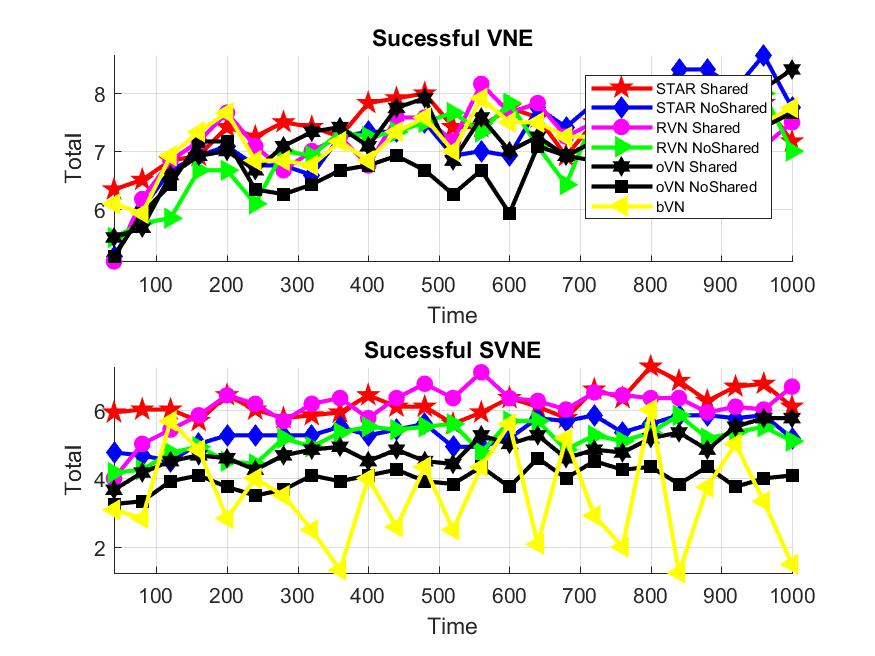
\includegraphics[width=4in]{figures/VirNetReqSurNetReq}\\
%  \caption{成功的VNE请求数和成功的SVNE请求数}\label{fig:VirNetReqSurNetReq}
%\end{figure}
%\begin{figure}[htbp]
%  \centering
%  % Requires \usepackage{graphicx}
%  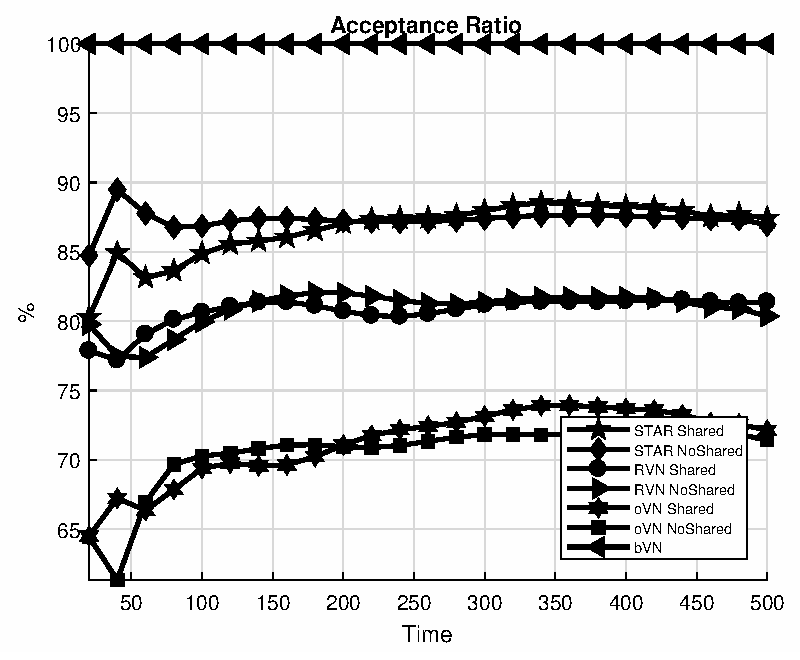
\includegraphics[width=4in]{figures/AcceptionRatio}\\
%  \caption{接受率}\label{fig:AcceptionRatio}
%\end{figure}

\begin{figure}[htbp]
\centering
\begin{minipage}{0.4\textwidth}
\centering
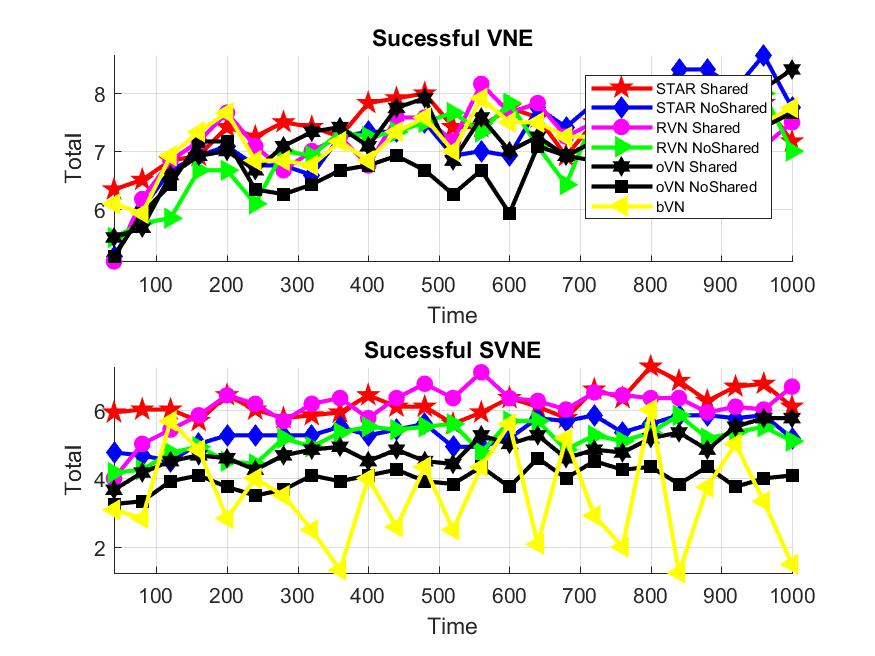
\includegraphics[width=\textwidth]{figures/VirNetReqSurNetReq}
\caption{成功的VNE请求数和成功的SVNE请求数}\label{fig:VirNetReqSurNetReq}
\end{minipage}
\begin{minipage}{0.4\textwidth}
\centering
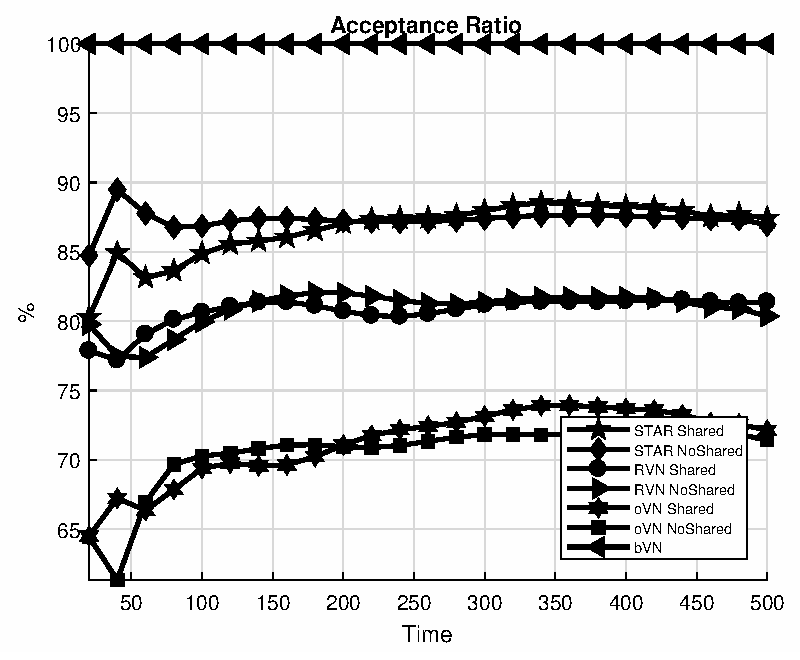
\includegraphics[width=\textwidth]{figures/AcceptionRatio}
\caption{接受率}\label{fig:AcceptionRatio}
\end{minipage}\vspace{\baselineskip}
\end{figure}

考虑所有虚拟节点的情况下,评估了SeVN问题启发式方法$\MyAlgorithmMethodAbrreviation$在分配资源时的性能。我们特别关注物理网络使用的资源和虚拟网络请求的资源情况,以及可生存虚拟网络请求的可接受率。
\section{算法性能评估及比较}
\subsection{接受率}
在这一部分中,如图\ref{fig:AcceptionRatio}所示比较了SeVN问题不同算法可生存性虚拟请求的接受率。此外,$\ThirdAlgorithmMethodAbrreviation$是所有其它算法前期的虚拟嵌入算法,在可生存性增广嵌入过程中,我们假设算法$\ThirdAlgorithmMethodAbrreviation$没有可生存性资源增广而已经达到可生存性功能需求。以$\ThirdAlgorithmMethodAbrreviation$作为标准比较算法来度量其它算法的性能,特别是可生存性需求导致的对底层物理网络额外资源消耗量。
%由于到达的VN请求没有足够的底层物理资源,在200次单元时间之前,接受率迅速下降。
如图\ref{fig:AcceptionRatio}所示,当系统中运行到250单元时间后接受率相对稳定和保持一致,$\MyAlgorithmMethodAbrreviation$ 算法比$\SecondAlgorithmMethodAbrreviation$ 算法有更高的接受率,接受率提高了近4\%,这是因为$\MyAlgorithmMethodAbrreviation$算法当可生存性需求时资源增广分配过程中比$\SecondAlgorithmMethodAbrreviation$ 算法消耗更少的底层资源。 $\MyAlgorithmMethodAbrreviation$-NoShared 比$\MyAlgorithmMethodAbrreviation$-Shared的接受率低,直观地说,这是因为$\MyAlgorithmMethodAbrreviation$-NoShared的为了可生存性的保证而需要更多的资源,备份资源之间都相互不共享,为了可生存性需求而资源增广都需要申请大量的额外资源,由于冗余资源消耗的原因,接受率至少比$\MyAlgorithmMethodAbrreviation$-Shared 损失了6\%。

\subsection{活动节点}
为了承载所有虚拟网络而需要使用的逻辑节点数如图\ref{fig:ActiveNodeAverageVirtualNetwork}所示,$\MyAlgorithmMethodAbrreviation$ 算法比其它算法使用更少的虚拟节点数这将使得$\MyAlgorithmMethodAbrreviation$ 算法比其它算法消耗更少的底层资源。

如图\ref{fig:ActiveNodeAverageSubstrateNetwork}所示,为了承载所有虚拟网络而需要启动和被嵌入虚拟节点的底层物理网络节点数,底层物理网络需要启动节点数与底层物理网络上承接的虚拟网络路径的平均长度有关,因为使用额外的节点来转发端节点之间的通信数据,因此,选择未启动的节点来转发数据的概率增加了。在能源效率方面,嵌入所需的底层物理网络节点数可以粗略估计能源消耗。
%\begin{figure}[htbp]
%  \centering
%  % Requires \usepackage{graphicx}
%  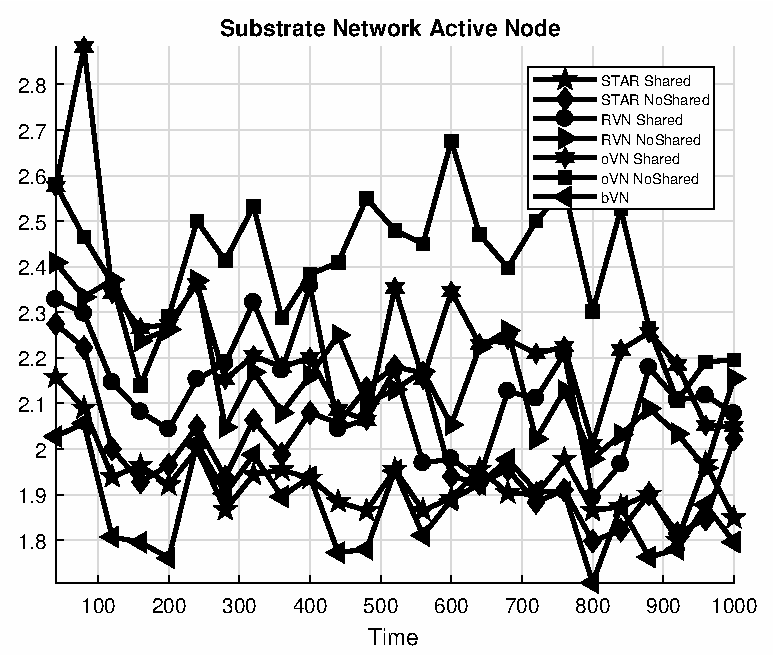
\includegraphics[width=4in]{figures/ActiveNodeAverageSubstrateNetwork}\\
%  \caption{底层物理网络平均启动的节点数}\label{fig:ActiveNodeAverageSubstrateNetwork}
%\end{figure}
%\begin{figure}[htbp]
%  \centering
%  % Requires \usepackage{graphicx}
%  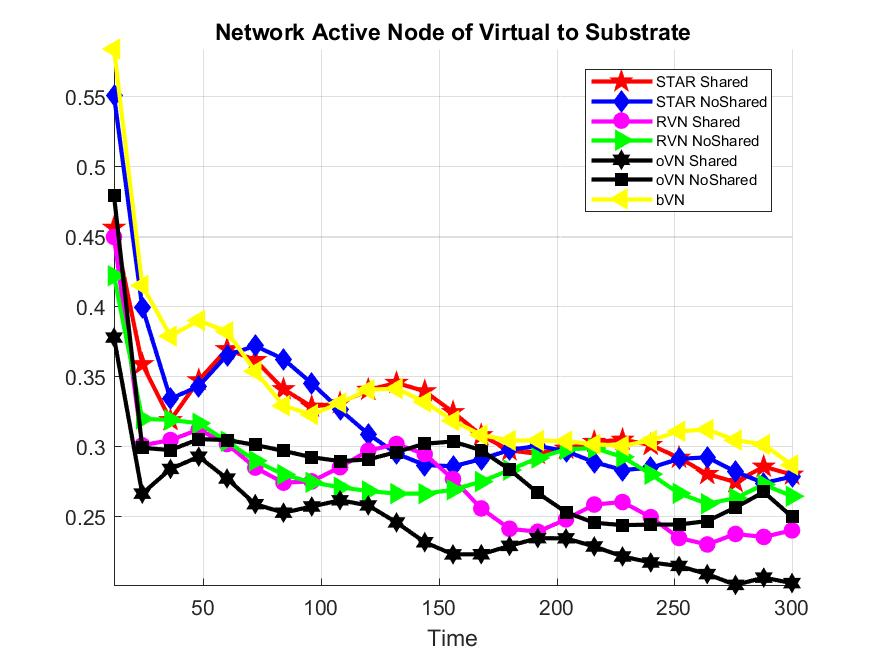
\includegraphics[width=4in]{figures/ActiveNodeSubVir2VirNet}\\
%  \caption{底层物理网络启动的节点数与虚拟网络虚拟节点数之比}\label{fig:ActiveNodeSubVir2VirNet}
%\end{figure}
%\begin{figure}[htbp]
%  \centering
%  % Requires \usepackage{graphicx}
%  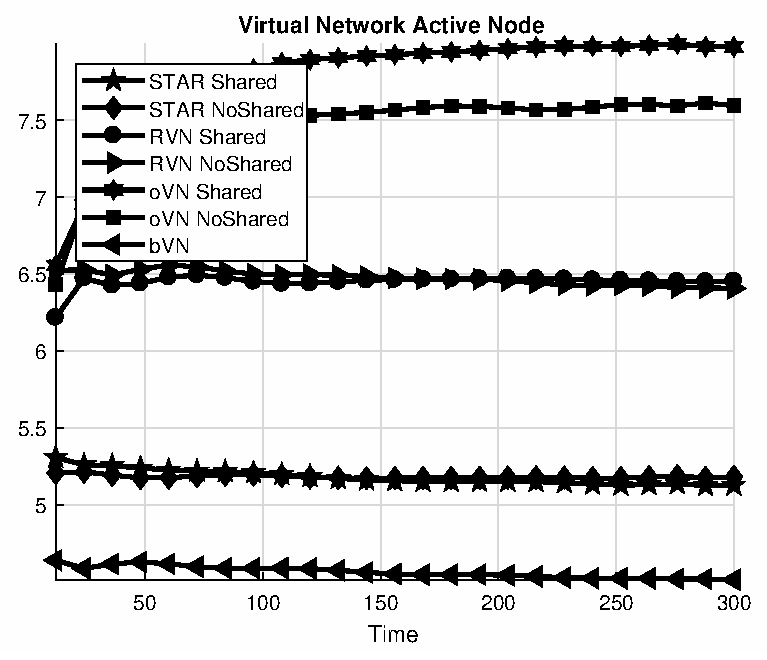
\includegraphics[width=4in]{figures/ActiveNodeAverageVirtualNetwork}\\
%  \caption{虚拟网络的平均虚拟节点数}\label{fig:ActiveNodeAverageVirtualNetwork}
%\end{figure}

\begin{figure}[htbp]
\centering
\begin{minipage}{0.4\textwidth}
\centering
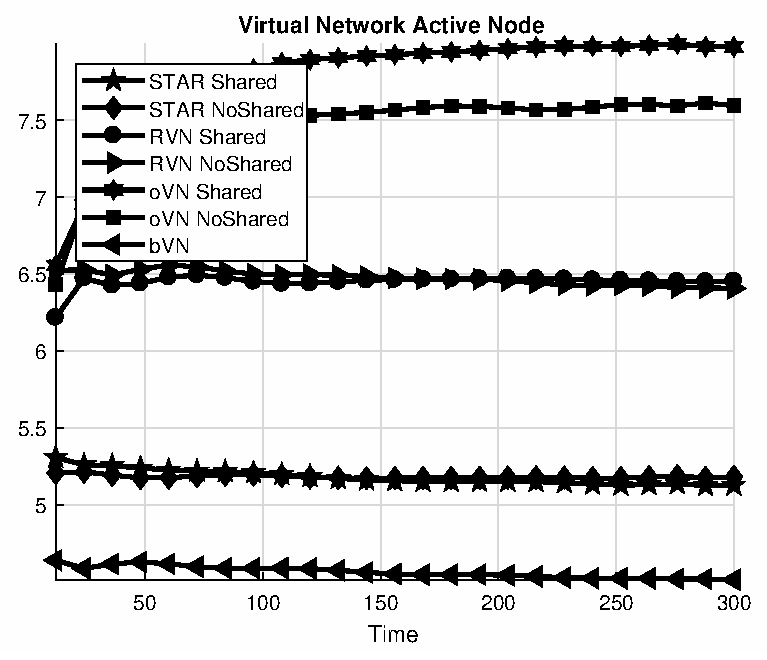
\includegraphics[width=\textwidth]{figures/ActiveNodeAverageVirtualNetwork}
\caption{虚拟网络的平均虚拟节点数}\label{fig:ActiveNodeAverageVirtualNetwork}
\end{minipage}
\begin{minipage}{0.4\textwidth}
\centering
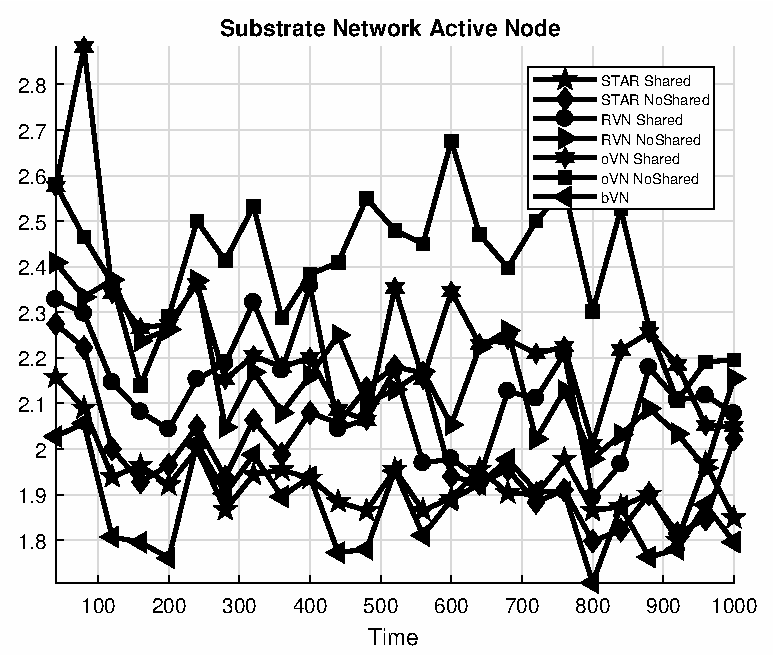
\includegraphics[width=\textwidth]{figures/ActiveNodeAverageSubstrateNetwork}
\caption{底层物理网络平均启动的节点数}\label{fig:ActiveNodeAverageSubstrateNetwork}
\end{minipage}
\begin{minipage}{0.4\textwidth}
\centering
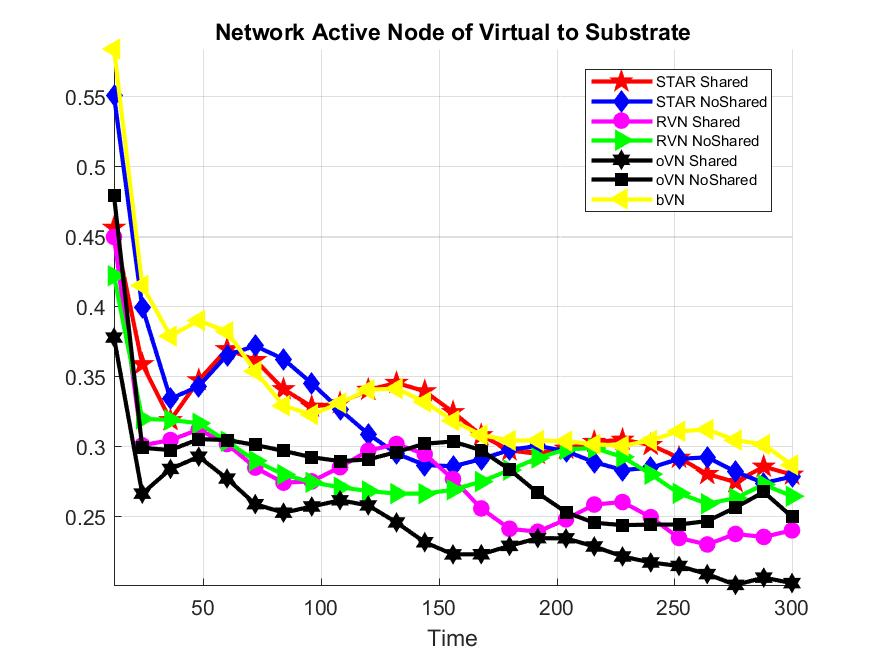
\includegraphics[width=\textwidth]{figures/ActiveNodeSubVir2VirNet}
\caption{底层物理网络启动的节点数与虚拟网络虚拟节点数之比}\label{fig:ActiveNodeSubVir2VirNet}
\end{minipage}\vspace{\baselineskip}
\end{figure}
底层物理网络启动的节点数与虚拟网络的虚拟节点数之比如图\ref{fig:ActiveNodeSubVir2VirNet}所示。


\subsection{链路与路径长度}
为了承载所有虚拟网络而需要使用的虚拟链路数如图\ref{fig:PathLengthAverageVirtualNetwork}所示,虚拟网络链路对应的物理路径越长,就需要为嵌入虚拟链路预留更多的资源。由于作为路径的一部分所以每个底层物理网络节点(接收节点除外)都需要一些时间来转发通过该路径发送的包,因此服务质量受路径长度的影响。通常,包延迟随着路径长度的增加而增加。

为了承载所有虚拟网络而需要使用的底层物理网络链路数如图\ref{fig:PathLengthAverageSubstrateNetwork}所示。
%\begin{figure}[htbp]
%  \centering
%  % Requires \usepackage{graphicx}
%  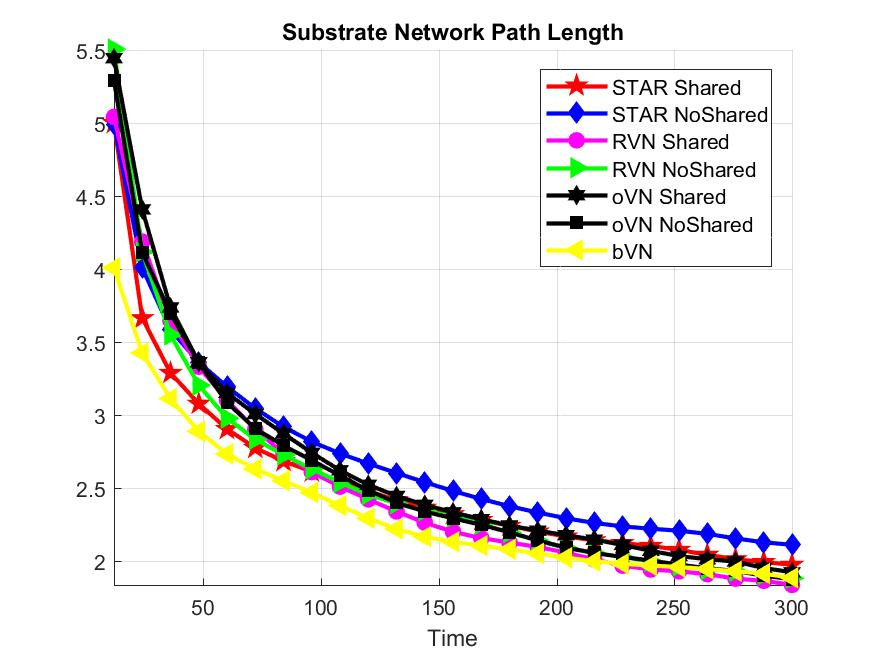
\includegraphics[width=4in]{figures/PathLengthAverageSubstrateNetwork}\\
%  \caption{物理网络链路数}\label{fig:PathLengthAverageSubstrateNetwork}
%\end{figure}
物理网络链路数与虚拟网络链路数之比如图\ref{fig:PathLengthSubVir2VirNet}所示。
%\begin{figure}[htbp]
%  \centering
%  % Requires \usepackage{graphicx}
%  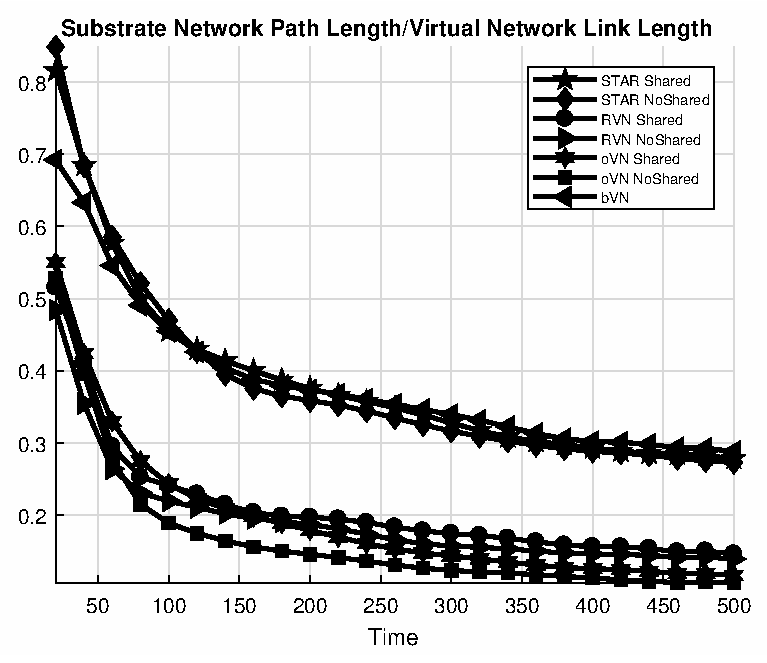
\includegraphics[width=4in]{figures/PathLengthSubVir2VirNet}\\
%  \caption{物理网络链路数与虚拟网络链路数之比}\label{fig:PathLengthSubVir2VirNet}
%\end{figure}
%\begin{figure}[htbp]
%  \centering
%  % Requires \usepackage{graphicx}
%  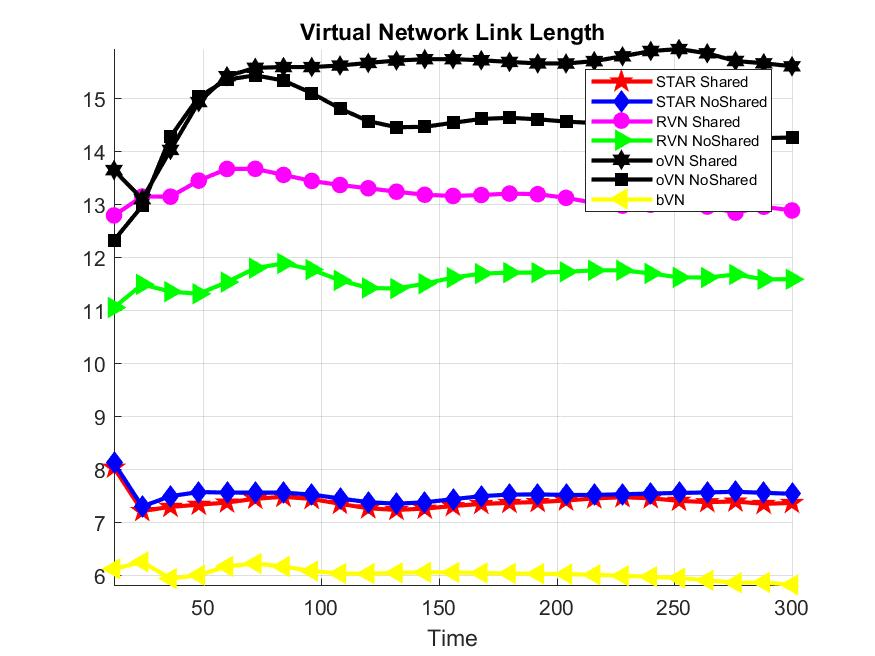
\includegraphics[width=4in]{figures/PathLengthAverageVirtualNetwork}\\
%  \caption{虚拟网络链路数}\label{fig:PathLengthAverageVirtualNetwork}
%\end{figure}
\begin{figure}[htbp]
\centering
\begin{minipage}{0.4\textwidth}
\centering
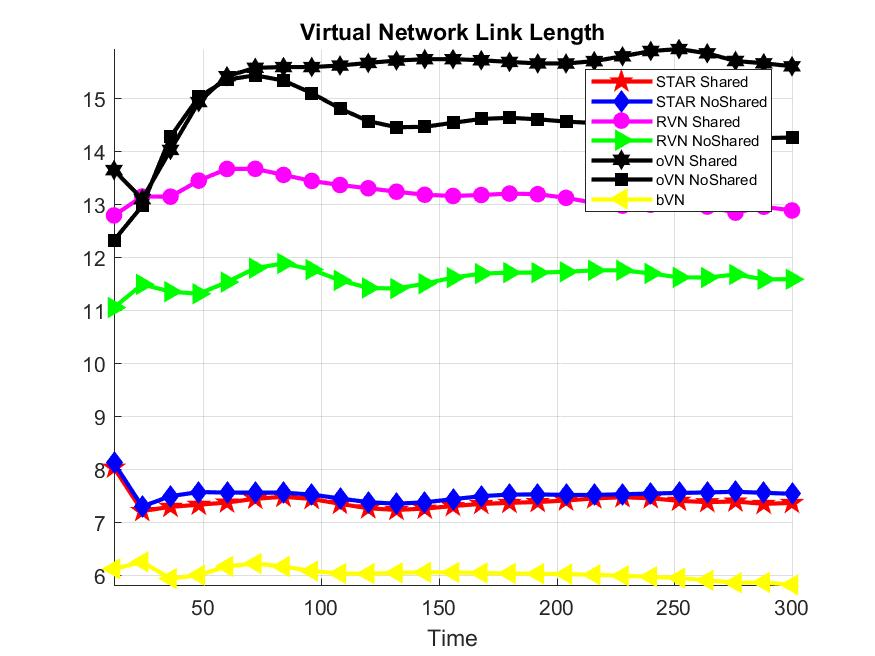
\includegraphics[width=\textwidth]{figures/PathLengthAverageVirtualNetwork}
\caption{虚拟网络链路数}\label{fig:PathLengthAverageVirtualNetwork}
\end{minipage}
\begin{minipage}{0.4\textwidth}
\centering
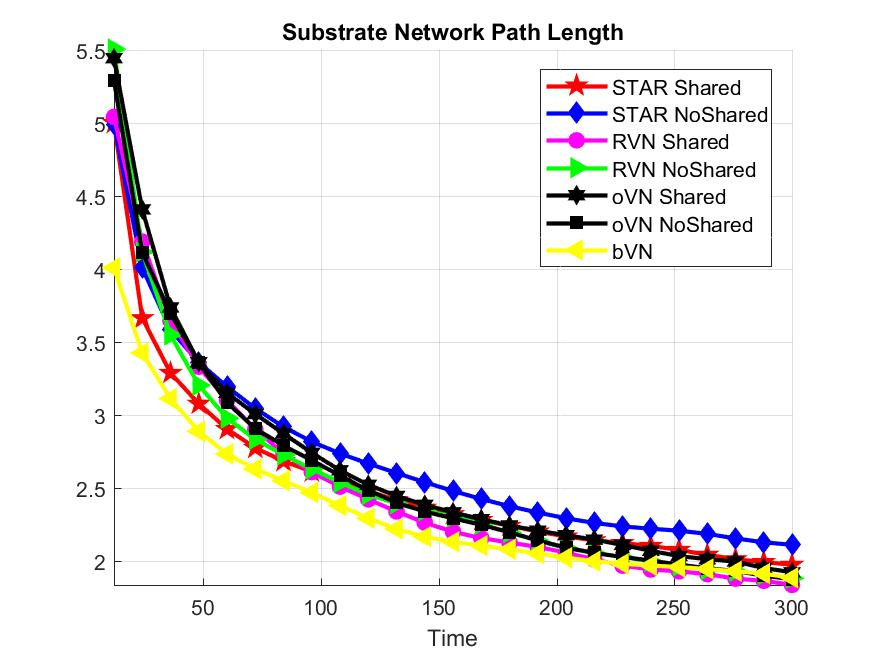
\includegraphics[width=\textwidth]{figures/PathLengthAverageSubstrateNetwork}
\caption{物理网络链路数}\label{fig:PathLengthAverageSubstrateNetwork}
\end{minipage}
\begin{minipage}{0.4\textwidth}
\centering
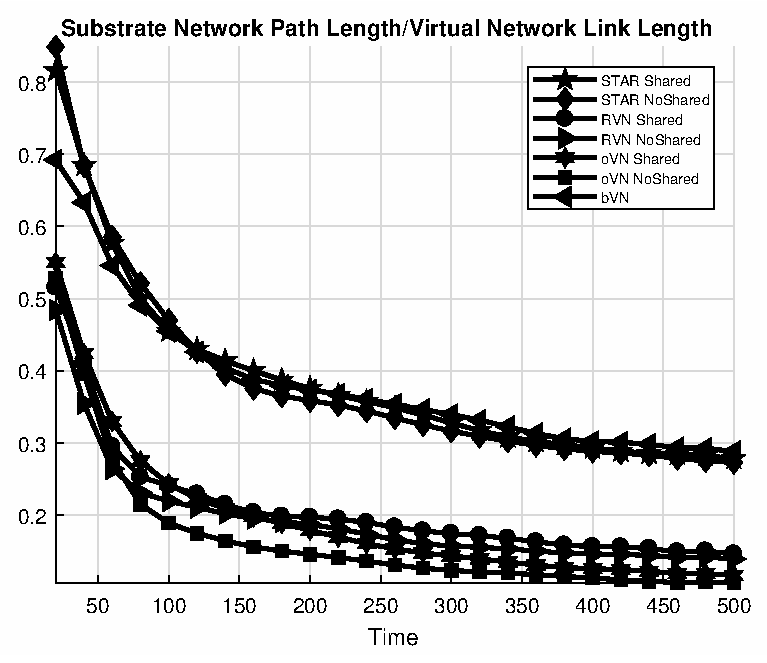
\includegraphics[width=\textwidth]{figures/PathLengthSubVir2VirNet}
\caption{物理网络链路数与虚拟网络链路数之比}\label{fig:PathLengthSubVir2VirNet}
\end{minipage}\vspace{\baselineskip}
\end{figure}
我提出的算法$\MyAlgorithmMethodAbrreviation$ 获得的虚拟网络链路数和物理网络链路数与算法$\ThirdAlgorithmMethodAbrreviation$最接近,算法$\MyAlgorithmMethodAbrreviation$比其它算法$\SecondAlgorithmMethodAbrreviation$和$\FouthAlgorithmMethodAbrreviation$ 具有更优的虚拟网络链路数和物理网络链路数。
\subsection{成本、收入和成本/收入比}
在本工作中,成本是为满足SEVN可生存性需求而消耗的底层物理资源(即所有底层物理设备节点的节点计算能力、所有光纤链路上的链路带宽)。
%底层物理网络实时消耗的成本如图\ref{fig:CostCurrentAverageSubstrateNetwork} 所示。
%\begin{figure}[htbp]
%  \centering
%  % Requires \usepackage{graphicx}
%  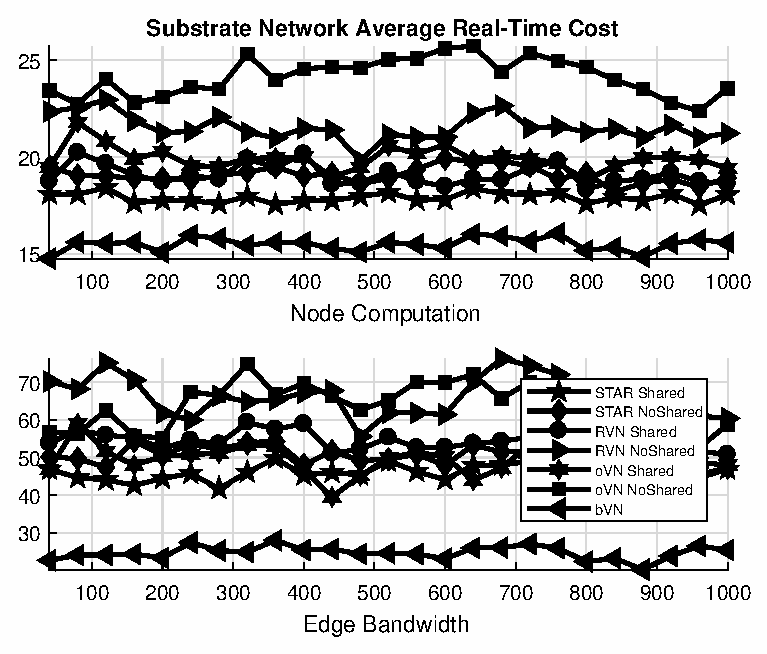
\includegraphics[width=4in]{figures/CostCurrentAverageSubstrateNetwork}\\
%  \caption{底层物理网络实时消耗的成本}\label{fig:CostCurrentAverageSubstrateNetwork}
%\end{figure}
底层物理网络消耗资源的平均成本如图\ref{fig:CostAccumulateAverageSubstrateNetwork}所示。
\begin{figure}[htbp]
\centering
\begin{minipage}{0.4\textwidth}
\centering
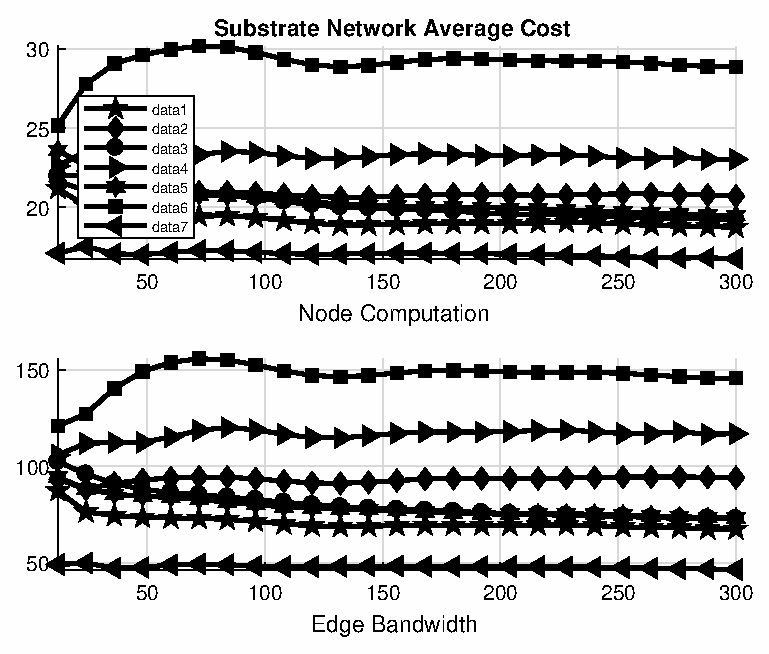
\includegraphics[width=\textwidth]{figures/CostAccumulateAverageSubstrateNetwork}
\caption{底层物理网络消耗资源的平均成本}\label{fig:CostAccumulateAverageSubstrateNetwork}
\end{minipage}
\begin{minipage}{0.4\textwidth}
\centering
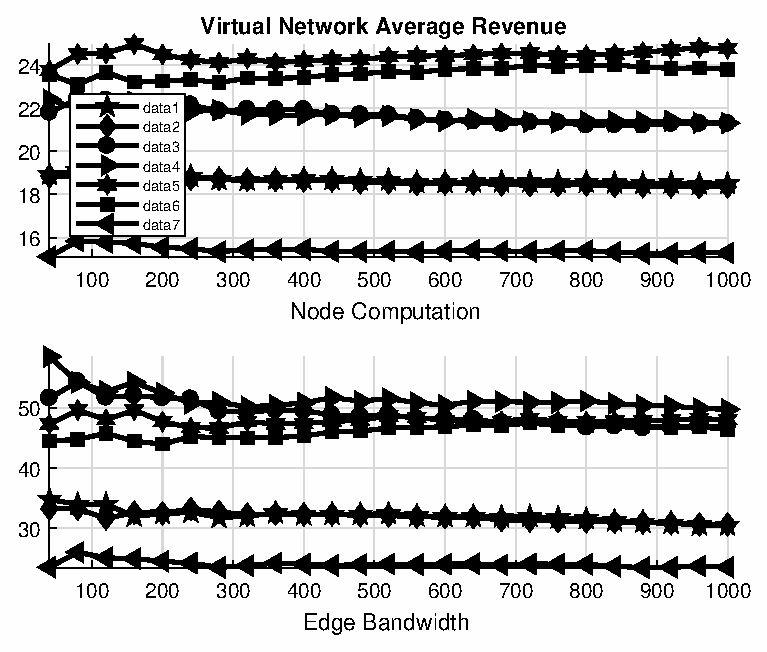
\includegraphics[width=\textwidth]{figures/RevenueAccumulateAverageVirtualNetwork}
\caption{虚拟网络获得需求的平均收益}\label{fig:RevenueAccumulateAverageVirtualNetwork}
\end{minipage}\vspace{\baselineskip}
\end{figure}
%\begin{figure}[htbp]
%  \centering
%  % Requires \usepackage{graphicx}
%  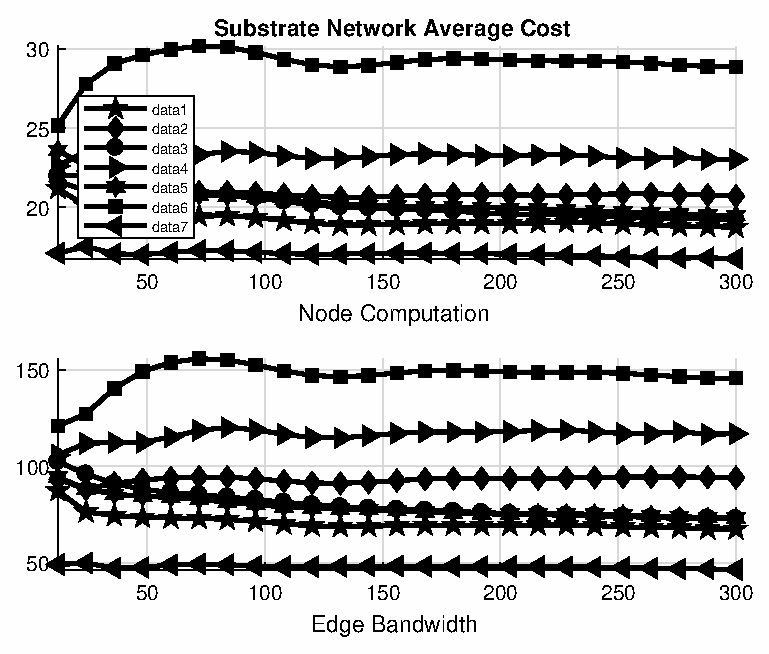
\includegraphics[width=4in]{figures/CostAccumulateAverageSubstrateNetwork}\\
%  \caption{底层物理网络消耗资源的平均成本}\label{fig:CostAccumulateAverageSubstrateNetwork}
%\end{figure}
%\begin{figure}[htbp]
%  \centering
%  % Requires \usepackage{graphicx}
%  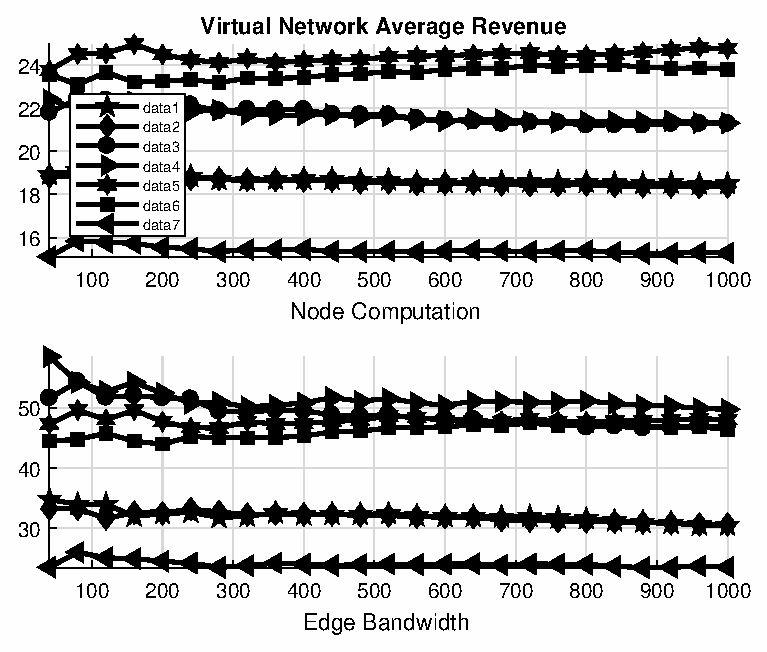
\includegraphics[width=4in]{figures/RevenueAccumulateAverageVirtualNetwork}\\
%  \caption{虚拟网络获得需求的平均收益}\label{fig:RevenueAccumulateAverageVirtualNetwork}
%\end{figure}
我提出的算法$\MyAlgorithmMethodAbrreviation$ 获得的成本和收益与算法$\ThirdAlgorithmMethodAbrreviation$最接近,算法$\MyAlgorithmMethodAbrreviation$比其它算法$\SecondAlgorithmMethodAbrreviation$和$\FouthAlgorithmMethodAbrreviation$ 具有更优的成本和收益。
%虚拟网络实时的平均收益如图\ref{fig:RevenueAverageCurrentVirtualNetwork} 所示。
%\begin{figure}[htbp]
%  \centering
%  % Requires \usepackage{graphicx}
%  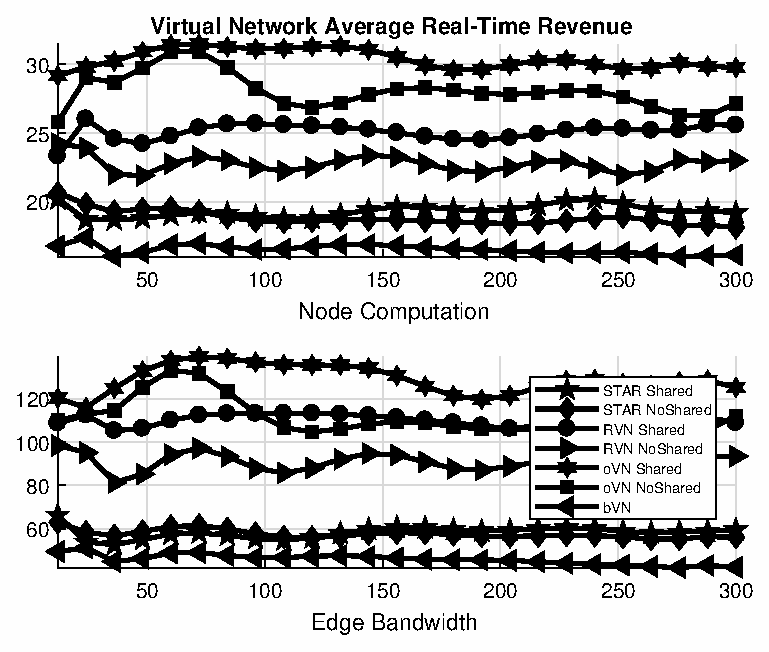
\includegraphics[width=4in]{figures/RevenueAverageCurrentVirtualNetwork}\\
%  \caption{虚拟网络实时的平均收益}\label{fig:RevenueAverageCurrentVirtualNetwork}
%\end{figure}
虚拟网络的平均收益如图\ref{fig:RevenueAccumulateAverageVirtualNetwork}所示。


%\subsection{压力}
%\subsection{迁移频率比}
%\subsection{效用}
%\subsection{备份节点数}

\section{小结}
本节提出了一种有效的算法$\MyAlgorithmMethodAbrreviation$,用于解决在具有可生存性保证请求的嵌入虚拟网络中,通过冗余节点和链路来有效地分配SeVN问题的增广资源(启动新的物理节点、链路带宽或节点计算)。资源分配方法考虑的是冗余节点是被动的还是主动的,只要在从故障恢复时有充足的资源可用。由于一个物理基础设施(底层网络)承载多个VN,因此在VN之间共享冗余节点是更有效的资源。若要减少分配给可生存性保证的资源,请执行以下操作。我们引入了一种启发式方法来共享这些独立的和相关的故障类型,并在星型构造分解和动态规划的基础上实现了资源的最优分配。我们的算法采用了一种新的资源分配方法来减少新的启动主机,在有限的进程时间内最小化资源,而且即使问题的规模相对较小,线性规划也无法计算出最优解。仿真结果表明,该算法在节约资源、实现高接受率、高资源利用率和低启动节点数量等方面具有显著的效果。
